%An Open-Access Dataset of Hospitalized Cardiac Arrest Patients: Creation and Utilization for Machine Learning-based Predictions"
%"Curating and Employing an Open Access Dataset for Machine Learning Prediction of Inpatient Cardiac Arrests"
%$"A Novel Open Access Dataset for Predicting Cardiac Arrest Using Machine Learning Analysis"
%"Contribution and Application of a New Open-Access Dataset: Machine Learning Analysis for Predicting Inpatient Cardiac Arrest"
%"Introducing and Applying an Open-Access Da


%  LaTeX support: latex@mdpi.com 
%  For support, please attach all files needed for compiling as well as the log file, and specify your operating system, LaTeX version, and LaTeX editor.

%=================================================================
\documentclass[journal,article,submit,pdftex,moreauthors]{Definitions/mdpi} 
\usepackage{graphicx}
\usepackage{subcaption}
\usepackage[acronym]{glossaries}
%--------------------
% Class Options:
%--------------------
%----------
% journal
%----------
% Choose between the following MDPI journals:
% acoustics, actuators, addictions, admsci, adolescents, aerobiology, aerospace, agriculture, agriengineering, agrochemicals, agronomy, ai, air, algorithms, allergies, alloys, analytica, analytics, anatomia, animals, antibiotics, antibodies, antioxidants, applbiosci, appliedchem, appliedmath, applmech, applmicrobiol, applnano, applsci, aquacj, architecture, arm, arthropoda, arts, asc, asi, astronomy, atmosphere, atoms, audiolres, automation, axioms, bacteria, batteries, bdcc, behavsci, beverages, biochem, bioengineering, biologics, biology, biomass, biomechanics, biomed, biomedicines, biomedinformatics, biomimetics, biomolecules, biophysica, biosensors, biotech, birds, bloods, blsf, brainsci, breath, buildings, businesses, cancers, carbon, cardiogenetics, catalysts, cells, ceramics, challenges, chemengineering, chemistry, chemosensors, chemproc, children, chips, cimb, civileng, cleantechnol, climate, clinpract, clockssleep, cmd, coasts, coatings, colloids, colorants, commodities, compounds, computation, computers, condensedmatter, conservation, constrmater, cosmetics, covid, crops, cryptography, crystals, csmf, ctn, curroncol, cyber, dairy, data, ddc, dentistry, dermato, dermatopathology, designs, devices, diabetology, diagnostics, dietetics, digital, disabilities, diseases, diversity, dna, drones, dynamics, earth, ebj, ecologies, econometrics, economies, education, ejihpe, electricity, electrochem, electronicmat, electronics, encyclopedia, endocrines, energies, eng, engproc, entomology, entropy, environments, environsciproc, epidemiologia, epigenomes, est, fermentation, fibers, fintech, fire, fishes, fluids, foods, forecasting, forensicsci, forests, foundations, fractalfract, fuels, future, futureinternet, futurepharmacol, futurephys, futuretransp, galaxies, games, gases, gastroent, gastrointestdisord, gels, genealogy, genes, geographies, geohazards, geomatics, geosciences, geotechnics, geriatrics, grasses, gucdd, hazardousmatters, healthcare, hearts, hemato, hematolrep, heritage, higheredu, highthroughput, histories, horticulturae, hospitals, humanities, humans, hydrobiology, hydrogen, hydrology, hygiene, idr, ijerph, ijfs, ijgi, ijms, ijns, ijpb, ijtm, ijtpp, ime, immuno, informatics, information, infrastructures, inorganics, insects, instruments, inventions, iot, j, jal, jcdd, jcm, jcp, jcs, jcto, jdb, jeta, jfb, jfmk, jimaging, jintelligence, jlpea, jmmp, jmp, jmse, jne, jnt, jof, joitmc, jor, journalmedia, jox, jpm, jrfm, jsan, jtaer, jvd, jzbg, kidneydial, kinasesphosphatases, knowledge, land, languages, laws, life, liquids, literature, livers, logics, logistics, lubricants, lymphatics, machines, macromol, magnetism, magnetochemistry, make, marinedrugs, materials, materproc, mathematics, mca, measurements, medicina, medicines, medsci, membranes, merits, metabolites, metals, meteorology, methane, metrology, micro, microarrays, microbiolres, micromachines, microorganisms, microplastics, minerals, mining, modelling, molbank, molecules, mps, msf, mti, muscles, nanoenergyadv, nanomanufacturing,\gdef\@continuouspages{yes}} nanomaterials, ncrna, ndt, network, neuroglia, neurolint, neurosci, nitrogen, notspecified, %%nri, nursrep, nutraceuticals, nutrients, obesities, oceans, ohbm, onco, %oncopathology, optics, oral, organics, organoids, osteology, oxygen, parasites, parasitologia, particles, pathogens, pathophysiology, pediatrrep, pharmaceuticals, pharmaceutics, pharmacoepidemiology,\gdef\@ISSN{2813-0618}\gdef\@continuous pharmacy, philosophies, photochem, photonics, phycology, physchem, physics, physiologia, plants, plasma, platforms, pollutants, polymers, polysaccharides, poultry, powders, preprints, proceedings, processes, prosthesis, proteomes, psf, psych, psychiatryint, psychoactives, publications, quantumrep, quaternary, qubs, radiation, reactions, receptors, recycling, regeneration, religions, remotesensing, reports, reprodmed, resources, rheumato, risks, robotics, ruminants, safety, sci, scipharm, sclerosis, seeds, sensors, separations, sexes, signals, sinusitis, skins, smartcities, sna, societies, socsci, software, soilsystems, solar, solids, spectroscj, sports, standards, stats, std, stresses, surfaces, surgeries, suschem, sustainability, symmetry, synbio, systems, targets, taxonomy, technologies, telecom, test, textiles, thalassrep, thermo, tomography, tourismhosp, toxics, toxins, transplantology, transportation, traumacare, traumas, tropicalmed, universe, urbansci, uro, vaccines, vehicles, venereology, vetsci, vibration, virtualworlds, viruses, vision, waste, water, wem, wevj, wind, women, world, youth, zoonoticdis 
% For posting an early version of this manuscript as a preprint, you may use "preprints" as the journal. Changing "submit" to "accept" before posting will remove line numbers.

%---------
% article
%---------
% The default type of manuscript is "article", but can be replaced by: 
% abstract, addendum, article, book, bookreview, briefreport, casereport, comment, commentary, communication, conferenceproceedings, correction, conferencereport, entry, expressionofconcern, extendedabstract, datadescriptor, editorial, essay, erratum, hypothesis, interestingimage, obituary, opinion, projectreport, reply, retraction, review, perspective, protocol, shortnote, studyprotocol, systematicreview, supfile, technicalnote, viewpoint, guidelines, registeredreport, tutorial
% supfile = supplementary materials

%----------
% submit
%----------
% The class option "submit" will be changed to "accept" by the Editorial Office when the paper is accepted. This will only make changes to the frontpage (e.g., the logo of the journal will get visible), the headings, and the copyright information. Also, line numbering will be removed. Journal info and pagination for accepted papers will also be assigned by the Editorial Office.

%------------------
% moreauthors
%------------------
% If there is only one author the class option oneauthor should be used. Otherwise use the class option moreauthors.

%---------
% pdftex
%---------
% The option pdftex is for use with pdfLaTeX. Remove "pdftex" for (1) compiling with LaTeX & dvi2pdf (if eps figures are used) or for (2) compiling with XeLaTeX.

%=================================================================
% MDPI internal commands - do not modify
\firstpage{1} 
\makeatletter 
\setcounter{page}{\@firstpage} 
\makeatother
\pubvolume{1}
\issuenum{1}
\articlenumber{0}
\pubyear{2023}
\copyrightyear{2023}
%\externaleditor{Academic Editor: Firstname Lastname}
\datereceived{ } 
\daterevised{ } % Comment out if no revised date
\dateaccepted{ } 
\datepublished{ } 
%\datecorrected{} % For corrected papers: "Corrected: XXX" date in the original paper.
%\dateretracted{} % For corrected papers: "Retracted: XXX" date in the original paper.
\hreflink{https://doi.org/} % If needed use \linebreak
%\doinum{}
%\pdfoutput=1 % Uncommented for upload to arXiv.org

%=================================================================
% Add packages and commands here. The following packages are loaded in our class file: fontenc, inputenc, calc, indentfirst, fancyhdr, graphicx, epstopdf, lastpage, ifthen, float, amsmath, amssymb, lineno, setspace, enumitem, mathpazo, booktabs, titlesec, etoolbox, tabto, xcolor, colortbl, soul, multirow, microtype, tikz, totcount, changepage, attrib, upgreek, array, tabularx, pbox, ragged2e, tocloft, marginnote, marginfix, enotez, amsthm, natbib, hyperref, cleveref, scrextend, url, geometry, newfloat, caption, draftwatermark, seqsplit
% cleveref: load \crefname definitions after \begin{document}

%=================================================================
% Please use the following mathematics environments: Theorem, Lemma, Corollary, Proposition, Characterization, Property, Problem, Example, ExamplesandDefinitions, Hypothesis, Remark, Definition, Notation, Assumption
%% For proofs, please use the proof environment (the amsthm package is loaded by the MDPI class).

%=================================================================
% Full title of the paper (Capitalized)
% Bed head ticket analysis for predicting inpatient cardiac arrest with machine learning
\Title{An Open-Access Data Set of Hospitalized Cardiac Arrest Patients: Machine Learning-Based Predictions Using Clinical Documentation}

% MDPI internal command: Title for citation in the left column
\TitleCitation{Title}

% Author Orchid ID: enter ID or remove command
\newcommand{\orcidauthorA}{0000-0003-4021-6677} % Add \orcidA{} behind the author's name
\newcommand{\orcidauthorB}{0000-0002-2245-4527} % Add \orcidB{} behind the author's name
\newcommand{\orcidauthorC}{0000-0002-1635-7560} % Add \orcidC{} behind the author's name
\newcommand{\orcidauthorD}{0000-0001-6026-0929} % Add \orcidD{} behind the author's name

% Authors, for the paper (add full first names)
\Author{Lahiru Rajapaksha $^{1,\ddagger,*}$\orcidA{}, Sugandima Vidanagamachchi $^{1,\ddagger}$\orcidB{}, Sampath Gunawardena $^{2,\ddagger}$\orcidC{} and Vajira Thambawita $^{3,\ddagger,*}$\orcidD{}}

%\longauthorlist{yes}

% MDPI internal command: Authors, for metadata in PDF
\AuthorNames{Firstname Lastname, Firstname Lastname and Firstname Lastname}

% MDPI internal command: Authors, for citation in the left column
\AuthorCitation{Rajapaksha, L.; Vidanagamachchi, S.; Gunawardena, S.; Thambawita, V;}
% If this is a Chicago style journal: Lastname, Firstname, Firstname Lastname, and Firstname Lastname.

% Affiliations / Addresses (Add [1] after \address if there is only one affiliation.)
\address{%
$^{1}$ \quad Department of Computer Science, University of Ruhuna, Matara, Sri Lanka; \\
$^{2}$ \quad Faculty of Medicine, University of Ruhuna, Karapitiya, Sri Lanka.\\
$^{3}$ \quad SimulaMet,Oslo, Norway.}


% Contact information of the corresponding author
\corres{Correspondence: ltwrajapaksha@gmail.com (L.R);
vajira@simula.no (V.T)}
% Current address and/or shared authorship
% \firstnote{Current address: Affiliation 3.} 
\secondnote{These authors contributed equally to this work.}
% The commands \thirdnote{} till \eighthnote{} are available for further notes

%\simplesumm{} % Simple summary

%\conference{} % An extended version of a conference paper

% Abstract (Do not insert blank lines, i.e. \\) 
% \abstract{Cardiac arrest is a sudden loss of heart function with serious consequences. In developing counties, healthcare professionals use clinical documentation to track patient information. These data can be used to predict developing cardiac arrest. Contributing to the advancement of the research domain  The model achieved high accuracy using commonly recorded medical details. This approach is effective in identifying the risk of cardiac arrest in in-ward patients, even in the absence of electronic medical recording systems. The study evaluated 112 patients who were transferred from the Emergency Treatment Unit to the Cardiac Medical Ward. The developed model achieved 96\% accuracy in predicting the risk of developing cardiac arrest.}
\abstract{
Cardiac arrest is a sudden loss of heart function with serious consequences. In developing counties, healthcare professionals use clinical documentation to track patient information. These data can be used to predict developing cardiac arrest. To contribute to the advancement of the research domain, we are publishing the data set through open access. Based on this data set our work revolves around generating and utilizing synthetic data by harnessing the potential of synthetic data vaults. We conducted a series of experiments by employing state-of-the-art machine learning techniques. These experiments were aimed to assess the performance of our developed predictive model in identifying the likelihood of developing a cardiac arrest. This approach is effective in identifying the risk of cardiac arrest in inpatients, even in the absence of electronic medical recording systems. The study evaluated 112 patients who were transferred from the Emergency Treatment Unit to the Cardiac Medical Ward. The developed model achieved 96\% accuracy in predicting the risk of developing cardiac arrest. In conclusion, our study showcases the potential of leveraging clinical documentation and synthetic data to create robust predictive models for cardiac arrest. The outcome of this effort will provide valuable insights and tools for healthcare professionals to preemptively address this critical medical condition.
}


% Keywords
\keyword{Bed Head Ticket; Cardiac Arrest; Clinical Documents; Decision Tree Classification Model; Early Warning System; Deep Learning;  Developing Country; Machine Learning; Recurrent Neural Network (RNN)} 

%%%%%%%%%%%%%%%%%%%%%%%%%%%%%%%%%%%%%%%%%%
% Only for the journal Data
%\dataset{DOI number or link to the deposited data set if the data set is published separately. If the data set shall be published as a supplement to this paper, this field will be filled by the journal editors. In this case, please submit the data set as a supplement.}
%\datasetlicense{License under which the data set is made available (CC0, CC-BY, CC-BY-SA, CC-BY-NC, etc.)}


\begin{document}
% Acronyms
\newacronym{lstm}{LSTM}{Long Short-Term Memory}
\newacronym{cvd}{CVD}{Cardiovascular Diseases}
\newacronym{ews}{EWS}{Early Warning System}
\newacronym{rrt}{RRT}{Rapid Response Teams}
\newacronym{drt}{DRT}{Dedicated Resuscitation Teams}
\newacronym{lmic}{LMIC}{Low to Middle-Income Country}
\newacronym{hic}{HIC}{High-Income Countries}
\newacronym{bht}{BHT}{Bed Head Ticket}
\newacronym{thk}{THK}{Teaching Hospital, Karapitiya}
\newacronym{etu}{ETU}{Emergency Treatment Unit}
\newacronym{hr}{HR}{Heart Rate}
\newacronym{sbp}{SBP}{Systolic Blood Pressure}
\newacronym{dbp}{DBP}{Diastolic Blood Pressure}
\newacronym{rr}{RR}{Respiratory Rate}
\newacronym{bt}{BT}{Body Temperature}
\newacronym{spo2}{SpO2}{Oxygen Saturation}
\newacronym{fbs}{FBS}{Fasting Blood Sugar}
\newacronym{fhihd}{FHIHD}{Family History of Ischemic Heart Diseases}
\newacronym{dlcapm}{DLCAPM}{Deep-Learning Cardiac Arrest Prediction Model}
\newacronym{rnn}{RNN}{Recurrent Neural Network}
\newacronym{cda}{CDA}{Clinical Decision Analysis}
\newacronym{smote}{SMOTE}{Synthetic Minority Over-sampling Technique}
\newacronym{gcs}{GCS}{Glasgow Coma Scale}
\newacronym{svm}{SVM}{Support Vector Machine}
\newacronym{ppv}{PPV}{Positive Predictive Value}
\newacronym{npv}{NPV}{Negative Predictive Value}
\newacronym{tpr}{TPR}{True Positive Rate}
\newacronym{fpr}{FPR}{False Positive Rate}
\newacronym{roc}{ROC}{Receiver Operating Characteristic}
\newacronym{mews}{MEWS}{Modified Early Warning Score}
\newacronym{cart}{CART}{Cardiac Arrest Risk Triage Score}
\newacronym{news}{NEWS}{National Early Warning Score}
\newacronym{mdcalc}{MDCALC}{Medical Calculator}
\newacronym{gru}{GRU}{Gated Recurrent Unit}
\newacronym{cnn}{CNN}{Convolutional Neural Networks}
\newacronym{emr}{EMR}{Electronic Medical Records}


\section{Introduction}

Cardiac arrest often occurs due to dysfunction in the heart's conduction system, which can cause the heart to stop pumping blood. Ventricular fibrillation is the most common cause (65-80\% of cases) \cite{b1}. Various heart-related causes include coronary artery disease, cardiomyopathy, inherited conditions, congenital heart disease, heart valve disease, acute myocarditis, and conduction disorders like long QT syndrome. Many patients may not recognize or ignore symptoms, with chest pain being the most common.

The ischemic coronary illness causes over 70\% of cardiac arrests and is the leading cause of cardiac dysfunction. Risk factors include hypertension, hyperlipidemia, diabetes, smoking, age, and family history of coronary diseases \cite{b2}. In Sri Lanka, \gls{cvd} account for a high mortality rate of 534 deaths per 100,000 \cite{b3} and 22.64\% of total deaths \cite{b4}. Cardiac arrest risk is 20-30\% within the first 24 hours after a heart attack. Survival rates are around 25\%, even with proper medical treatment.

The time to receive help and treatment is crucial for survival in sudden cardiac arrest cases.\Gls{ews} and can help identify deteriorating patients at risk of death from cardiac arrest \cite{b5}. Patients who experienced sudden cardiac arrest and were admitted to the Intensive Care Unit (ICU) showed signs of deterioration hours before the event. Early detection and treatment can reduce mortality rates, and Early Warning System (\gls{ews}) is designed based on patients' vital signs to aid in this process \cite{b6}.
This study makes several important contributions by,
\begin{itemize}
    \item Publishing an Open Access bedhead ticket dataset.
    \item Introducing a machine learning model to predict the risk of fatal cardiac arrests, which has shown improved results.
    \item Analysing the data set with machine learning models to compare the usability of the dataset.
\end{itemize}
Repository links
\begin{itemize}
    \item \href{https://zenodo.org/record/7603772}{Dataset(Zenodo)}
    \item \href{https://github.com/LahiruRajapaksha/cardiac-arrest-prediction-using-bed-head-tickets.git}{Model(GitHub)} 
\end{itemize}
%%%%%%%%%%%%%%%%%%%%%%%%%%%%%%%%%%%%%%%%%%
\section{Materials and Methods}
\subsection{Methodology}
The research was designed as a retrospective cohort study, focusing on patients admitted to the cardiac ward between August 13th, 2018, and February 6th, 2020, at Teaching Hospital, Karapitiya (THK), Galle, Sri Lanka. The study population included patients who were transferred to the cardiac ward from the Emergency Treatment Unit (ETU), excluding other types of patients and pediatric patients. A total of 112 patients, aged 15-89 years, were included in the study, with 82 male patients and 30 female patients.

Ethical clearance was obtained from the Ethics Review Committee of the Faculty of Medicine, University of Ruhuna, Galle, Sri Lanka, and the study adhered to the relevant guidelines and regulations established by the committee. Permission to access data was granted by the Director of Teaching Hospital Karapitiya. As this was a retrospective study, obtaining informed consent from all subjects was not applicable.

Data collection involved extracting information from the \gls{bht} in the hospital's record room. Due to the absence of electronic clinical data, each \gls{bht} was manually examined to collect the necessary data. The \gls{bht} contained information on the patient's health status, clinical history, management actions, investigations, treatments, progress, and diagnosis.

The extracted \gls{bht} data were categorized into five main categories: demographic features, examinations, lab reports, patient history, and outcomes (Fig. \ref{fig:figure1}). The extracted features were further analyzed to determine their availability concerning patients' hospital stays. Features with an availability rate of over 60\% (Fig. \ref{fig:figure2}) were selected for model development.

\begin{figure}[hbt!]
    \centering
    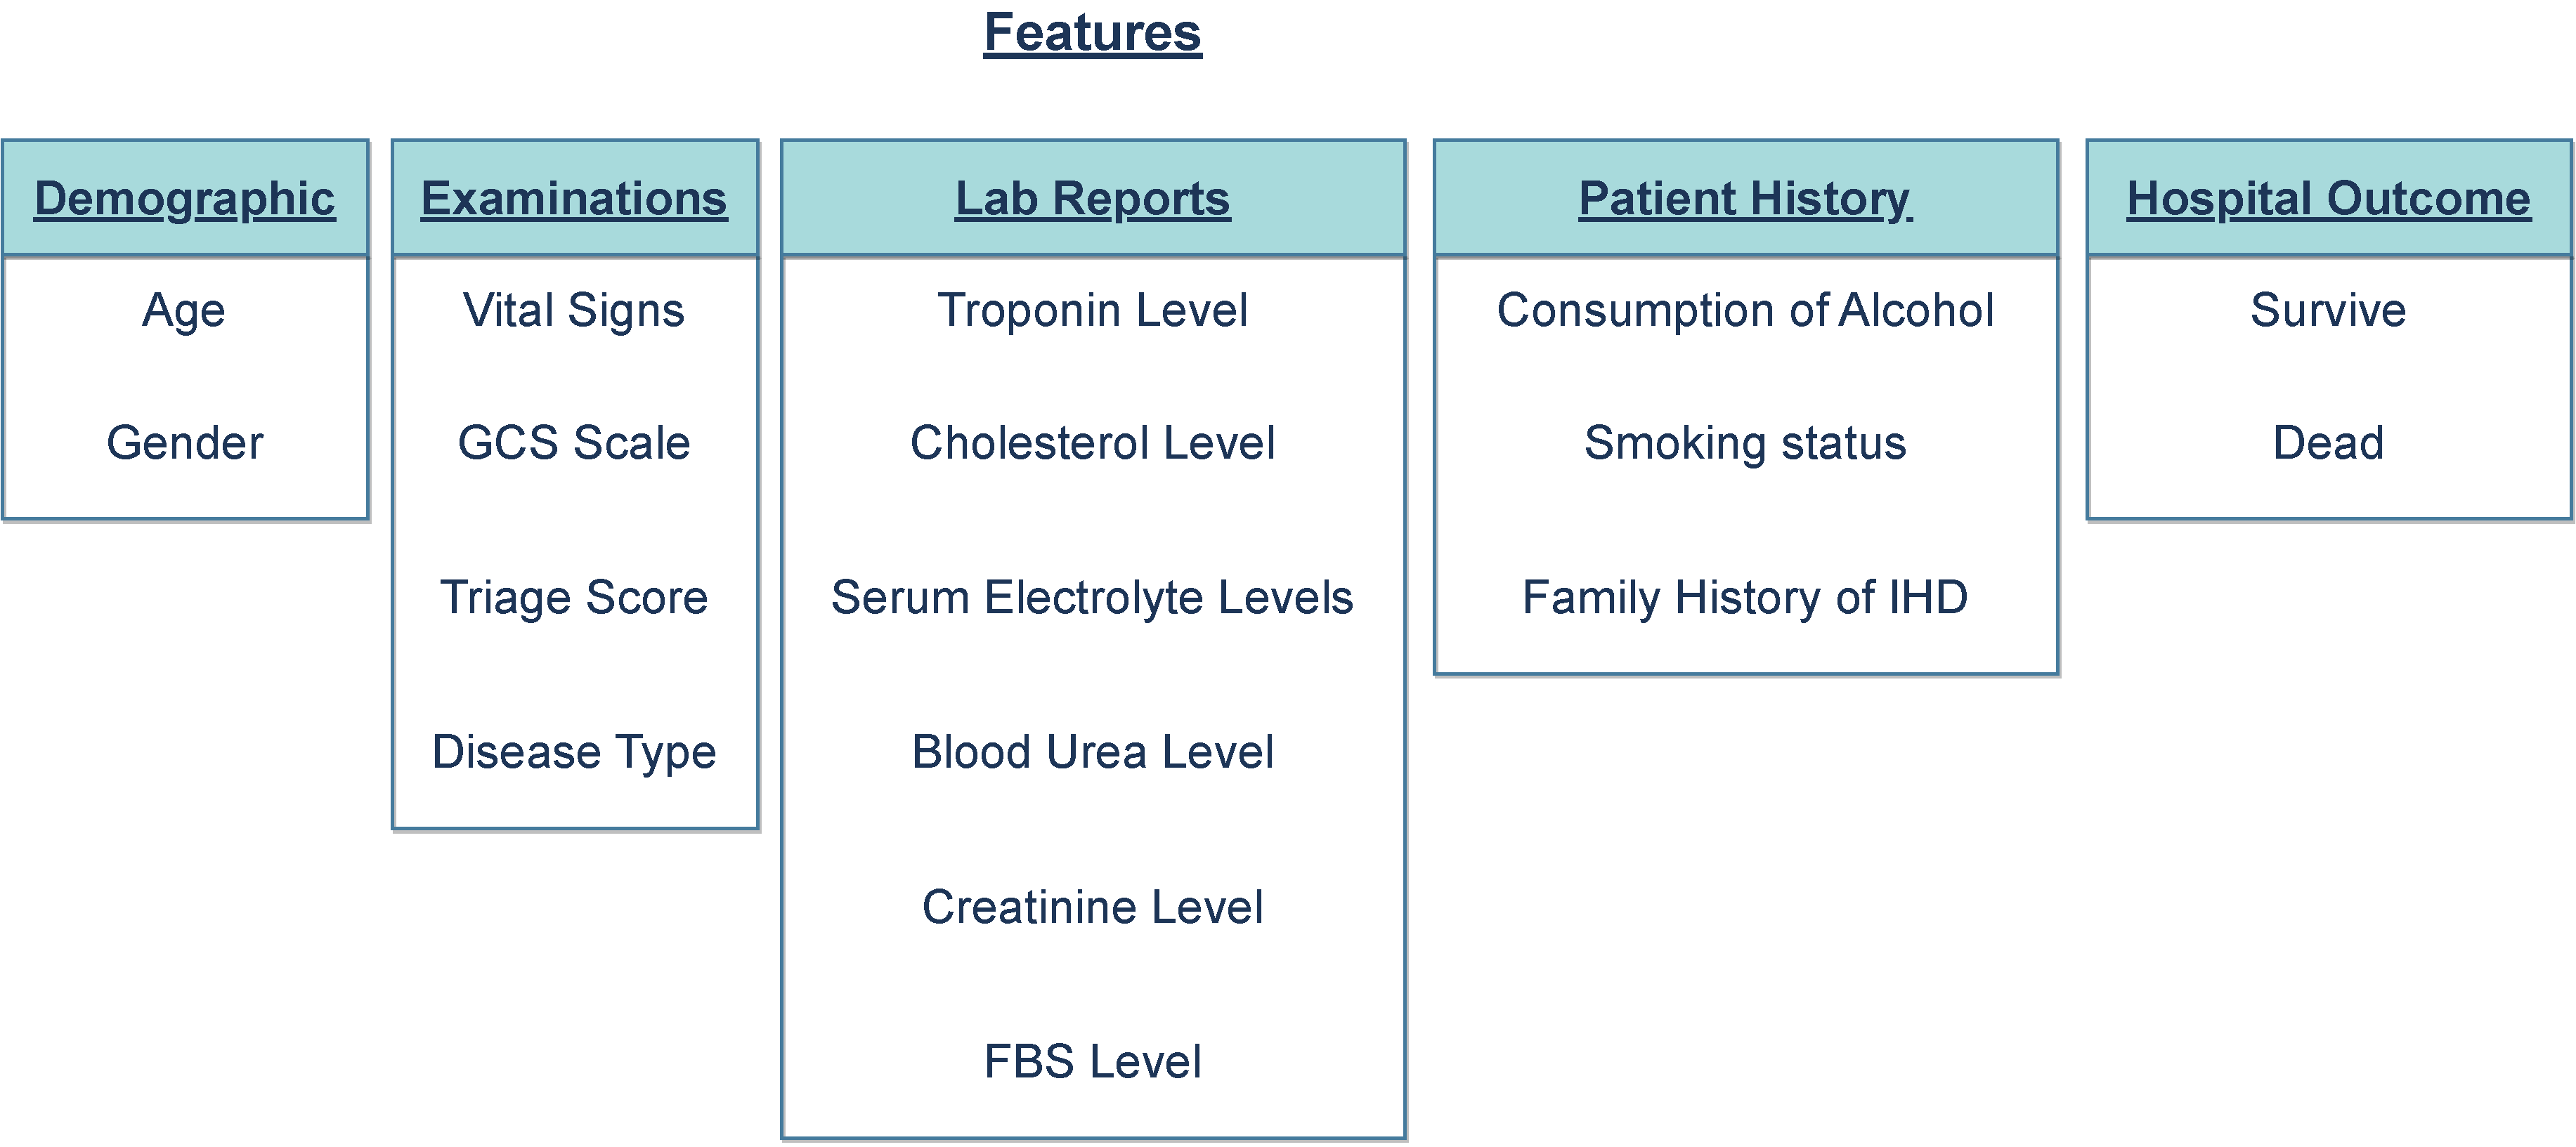
\includegraphics[width=1\linewidth]{images/featureCategorization.pdf}
    \caption{\textit{Categorization of extracted features into groups}}
    \label{fig:figure1}
    \vspace{-10pt}
\end{figure}

\begin{figure}[hbt!]
    \centering
    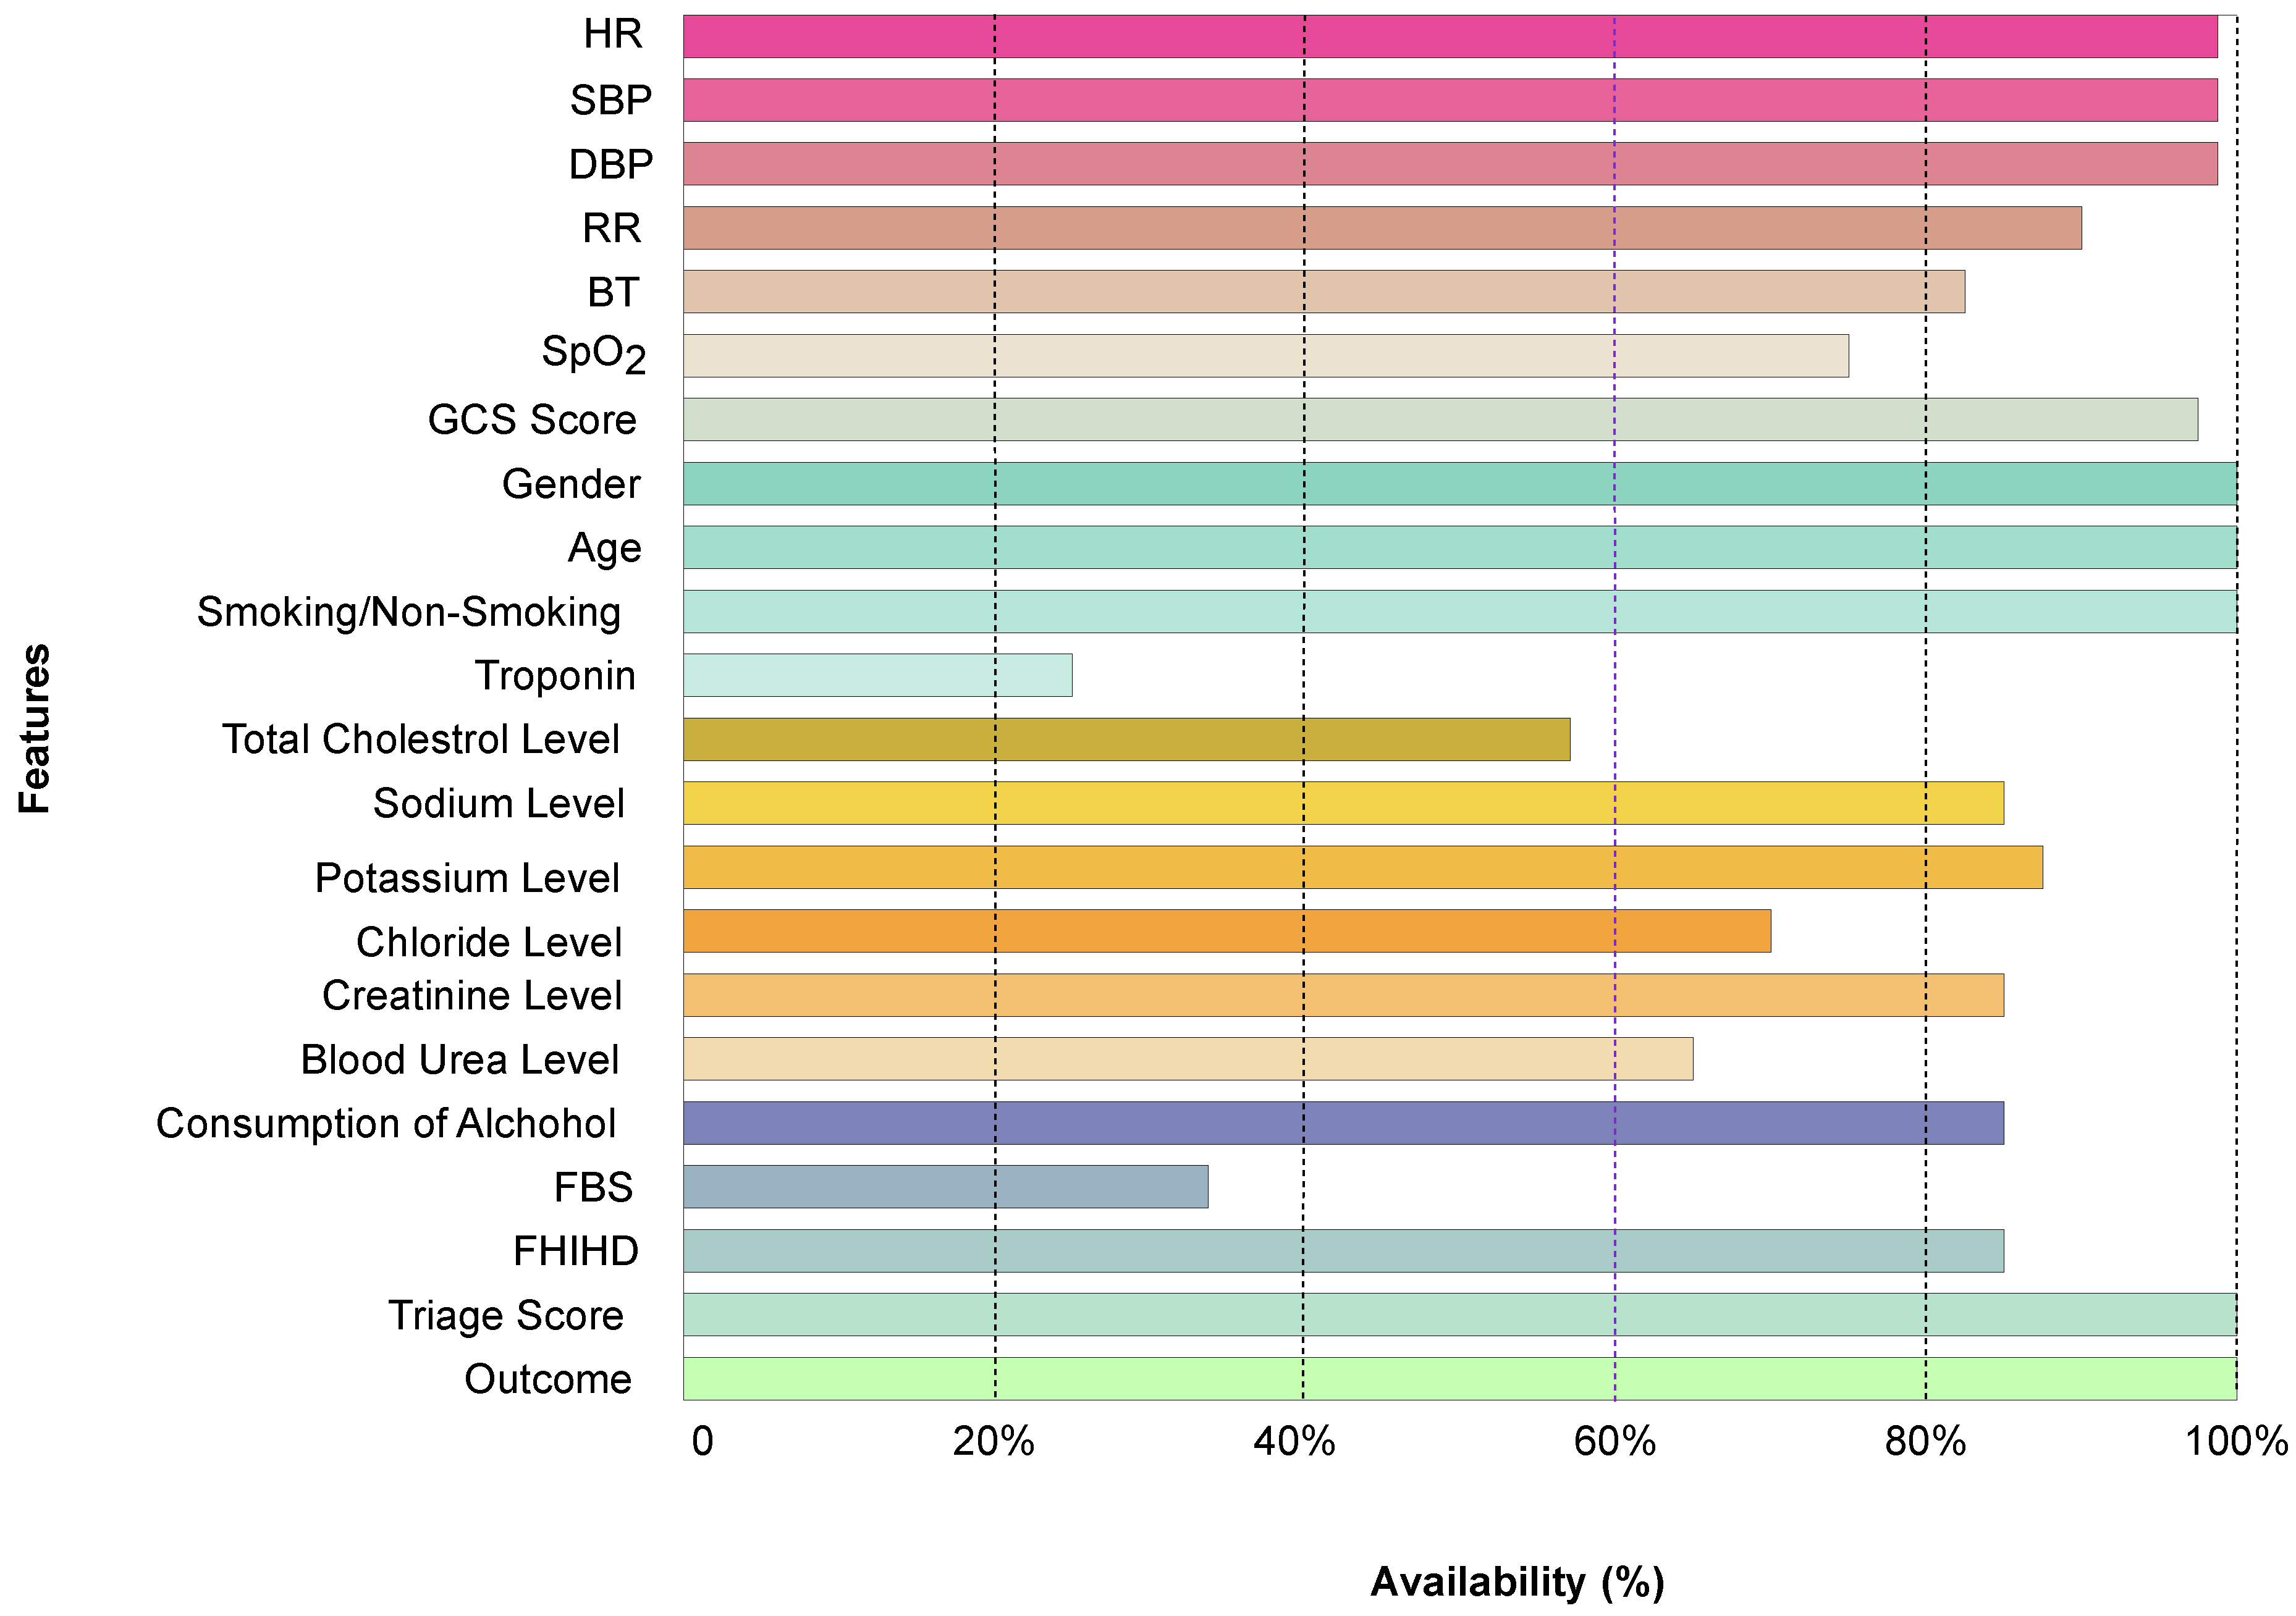
\includegraphics[width=1\linewidth]{images/featureAvailability.pdf}
    \caption{\textit{Feature availability of 112 patients}}
    \label{fig:figure2}
    \vspace{-10pt}
\end{figure}

\subsection{Data preprocessing}

As illustrated in Fig. \ref{fig:figure3}, the extracted clinical data were primarily divided into two categories: time-series data and non-time-series data. Time-series data consisted of patient information recorded in relation to time, while non-time-series data encompassed the remaining data. The clinical dataset contained 21 features: age, heart rate (HR), Systolic Blood Pressure (SBP), Diastolic Blood Pressure (DBP), Respiratory Rate (RR), Body Temperature (BT), Oxygen Saturation (SpO2), level of consciousness, troponin level, total cholesterol level, Fasting Blood Sugar level (FBS), serum electrolytes (Sodium, Potassium, Chloride), urea level, creatinine level, triage score (risk score on admission), alcohol consumption, smoking status, Family History of Ischemic Heart Diseases (FHIHD), and hospital outcome.

\begin{figure}[hbt!]
    \centering
    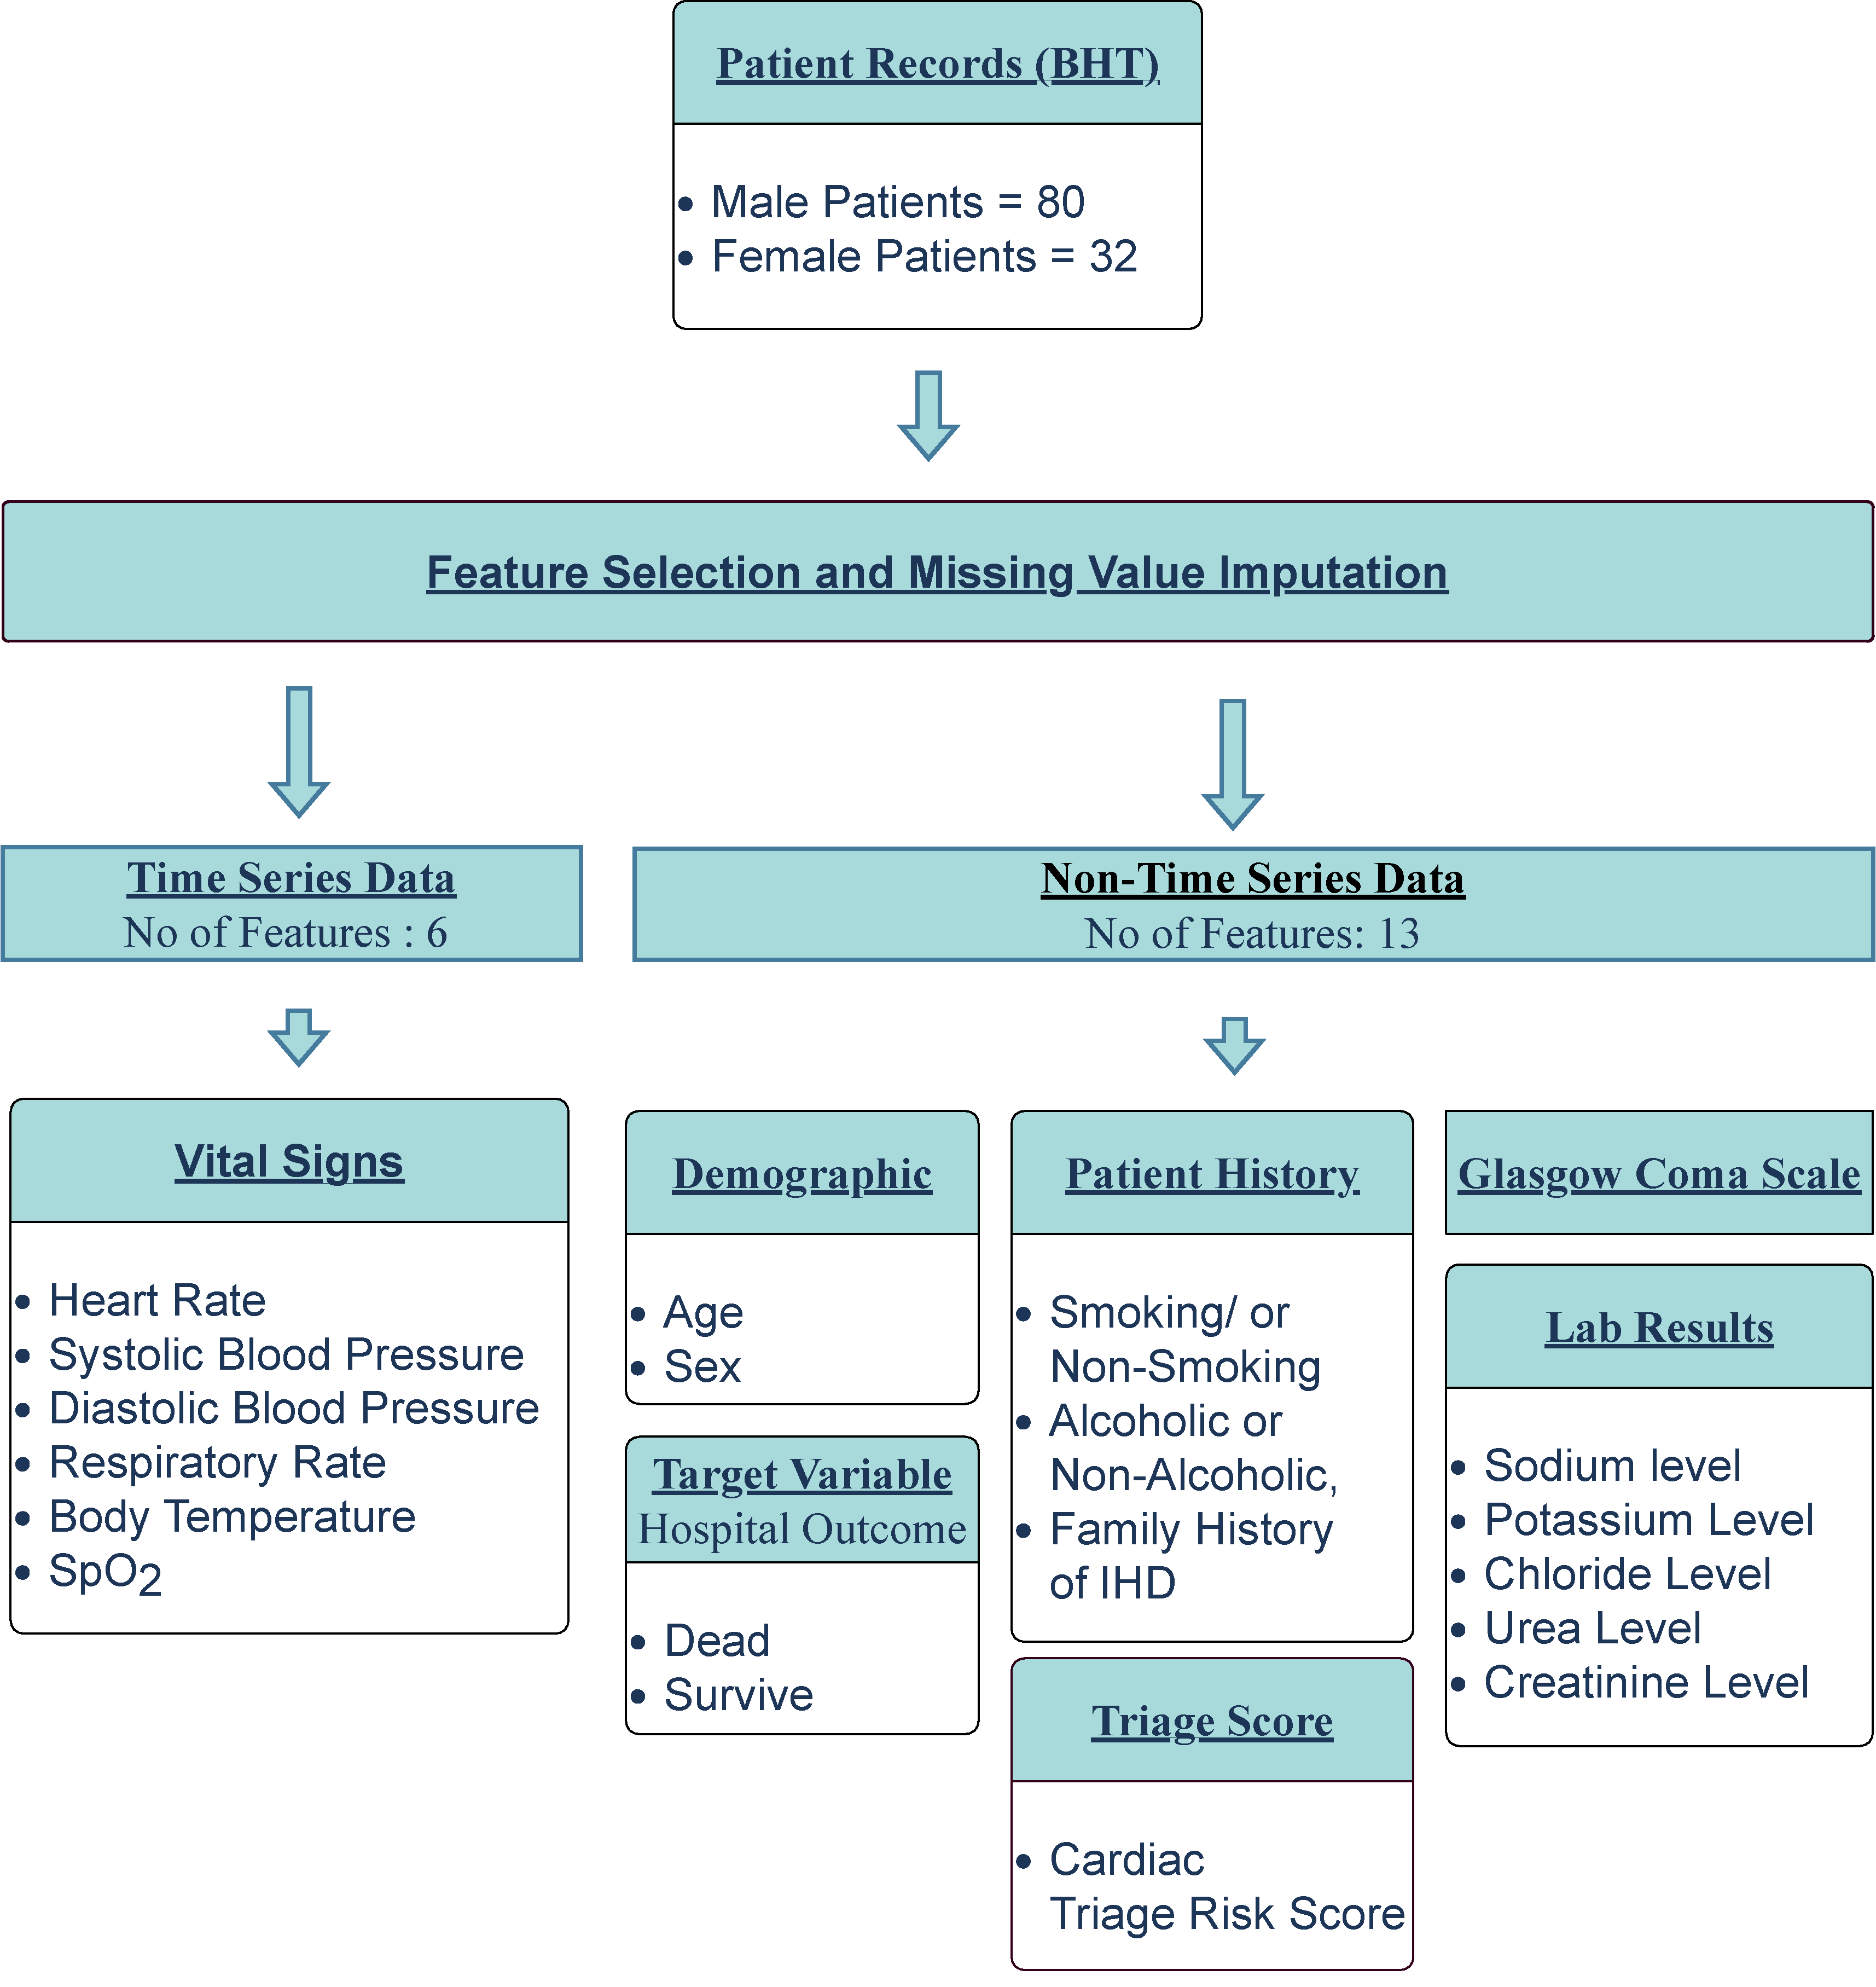
\includegraphics[width=0.75\linewidth]{images/dataPreprocessing.pdf}
    \caption{\textit{Data preprocessing workflow}}
    \label{fig:figure3}
    \vspace{-10pt}
\end{figure}

Out of the 21 features, 19 were selected for inclusion, while three were excluded from the final feature list. Troponin level, total cholesterol level, and fasting blood sugar level, which can be used to detect comorbidities in patients, were excluded due to insufficient records in the \glspl{bht} for the majority of patients. Data preprocessing consisted of two steps. First, 19 common features, including the patient's hospital outcome (target variable), were selected. Second, missing value imputation was performed for the selected features. If any feature data was missing, the most recent value was used; if no value was available, the median value was used.

Regarding time-series data (SBP, DBP, HR, RR, BT, SpO2), patients were monitored hourly throughout their hospital stay. In the selected data set, patients were monitored for a minimum of one hour and a maximum of 266 hours (11 days). A suitable time step (time window) for observation was chosen from this range. The time step was determined based on the average observation time of a patient (52 hours). This 52-hour observational time window is considered the prediction window of the model. For non-time-series data, only the results from the patient's lab tests conducted on the hospital admission date were considered.

\subsection{Data Division and Preparation}
After preprocessing the data set, we partitioned the data set into distinct three subsets to the ratio of 8:1:1, namely the training set, testing set, and validation set. Then the training data set is further enhanced through the infusion of synthetic data generated by Synthetic Data Valult (SDV) (Figure \ref{fig:figure4}). The goal of the SDV is to build generative models of relational databases \cite{a14}. By incorporating its capability of creating artificial instances that mimic the statistical properties of the original data set we expanded our training data, fostering greater diversity and aiding the model's ability to capture complex patterns.
\begin{figure}[hbt!]
    \centering
    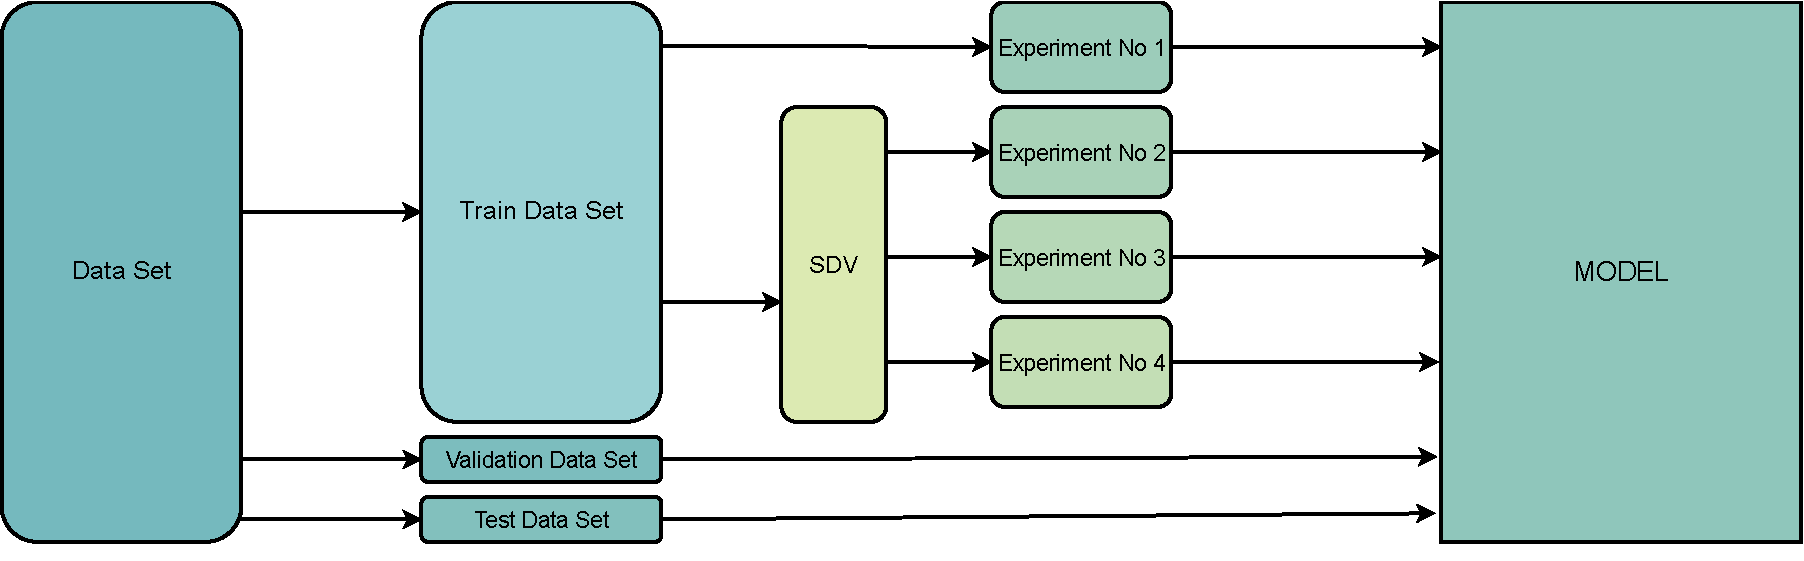
\includegraphics[width=\linewidth]{images/SDV.pdf}
    \caption{\textit{Data Division and preparation for the model}}
    \label{fig:figure4}
    \vspace{-10pt}
\end{figure}
When generating the synthetic data for experiments no 2-4, our consistent aim is to achieve a balanced ratio of survived patient data to dead patient data at 1:1, ensuring equal representation(Table \ref{tbl:data_division_table}).
\begin{table}[htbp]
\caption{Summary of the number of patient records and sequences contains in training data sets. Except for experiment No 01, we maintained the survived: dead ratio as 1:1 }
\resizebox{\columnwidth}{!}{%
\begin{tabular}{|l|cc|cc|cc|cc|}
\hline
\multirow{2}{*}{} &
  \multicolumn{2}{c|}{Training Data Set 01} &
  \multicolumn{2}{c|}{Training Data Set 02} &
  \multicolumn{2}{c|}{Training Data Set 03} &
  \multicolumn{2}{c|}{Training Data Set 04} \\ \cline{2-9} 
 &
  \multicolumn{1}{c|}{No of Sequences} &
  No of Records &
  \multicolumn{1}{c|}{No of Sequences} &
  No of Records &
  \multicolumn{1}{c|}{No of Sequences} &
  No of Records &
  \multicolumn{1}{c|}{No of Sequences} &
  No of Records \\ \hline
Real Survived Patients Data      & \multicolumn{1}{c|}{4287} & 74 & \multicolumn{1}{c|}{4287} & 74  & \multicolumn{1}{c|}{0}    & 0   & \multicolumn{1}{c|}{4287}  & 74  \\ \hline
Synthetic Survived Patients Data & \multicolumn{1}{c|}{0}    & 0  & \multicolumn{1}{c|}{0}    & 0   & \multicolumn{1}{c|}{4870} & 74  & \multicolumn{1}{c|}{4870}  & 74  \\ \hline
Real Dead Patients Data          & \multicolumn{1}{c|}{743}  & 15 & \multicolumn{1}{c|}{743}  & 15  & \multicolumn{1}{c|}{0}    & 0   & \multicolumn{1}{c|}{743}   & 15  \\ \hline
Synthetic Dead Patients Data     & \multicolumn{1}{c|}{0}    & 0  & \multicolumn{1}{c|}{1768} & 59  & \multicolumn{1}{c|}{4702} & 74  & \multicolumn{1}{c|}{5259}  & 133 \\ \hline
Total                            & \multicolumn{1}{c|}{5030} & 89 & \multicolumn{1}{c|}{6798} & 148 & \multicolumn{1}{c|}{9572} & 148 & \multicolumn{1}{c|}{15159} & 296 \\ \hline
\end{tabular}%
}
\label{tbl:data_division_table}
\end{table}


\subsection{Model architecture}

The integration of artificial intelligence into clinical practice has led to numerous studies focused on predicting adverse events, such as cardiac arrests before they occur. Evidence from these studies suggests that deep learning models are more efficient at identifying high-risk patients compared to existing \glspl{ews} \cite{b14}. \Gls{rnn} models are particularly well-suited for handling temporal sequence data. Among \gls{rnn} variants, \gls{lstm} has demonstrated remarkable performance in various sequence-based tasks \cite{b15}. Recent studies have also shown that deep learning models employing \gls{rnn} architectures with \gls{lstm} outperform clinical prediction models developed using logistic regression \cite{b16,b17}. Consequently, we chose the \gls{lstm} structure to model the temporal relationships within data extracted from the \gls{bht}.

\subsubsection{LSTM model}

The Deep-Learning Cardiac Arrest Prediction Model (DLCAPM) consists of a \gls{lstm} designed to handle time-series data, followed by a dense layer. During the model's development, we employed a sigmoid activation function for the dense layer, the Adam optimizer with default parameters, and binary-cross entropy as the loss function. The complete data set was divided into 30\% for validation and 70\% for training. Inputs to the \gls{lstm} model include Systolic Blood Pressure (SBP), Diastolic Blood Pressure (DBP), Heart Rate (HR), Respiratory Rate (RR), Body Temperature (BT), and Oxygen Saturation (SpO2) levels. The input data which was fed into the \gls{lstm} comprised a three-dimensional array of 112 × 52 × 6 (5824 patient record instances), as illustrated in Fig \ref{fig:figure5}. The first phase of the model aimed to handle temporal data, while the second phase combined the results of the time-series data with non-time-series data. This combined data was then input into the decision tree model to predict the final outcome based on the model's results.

\begin{figure}[hbt!]
    \centering
    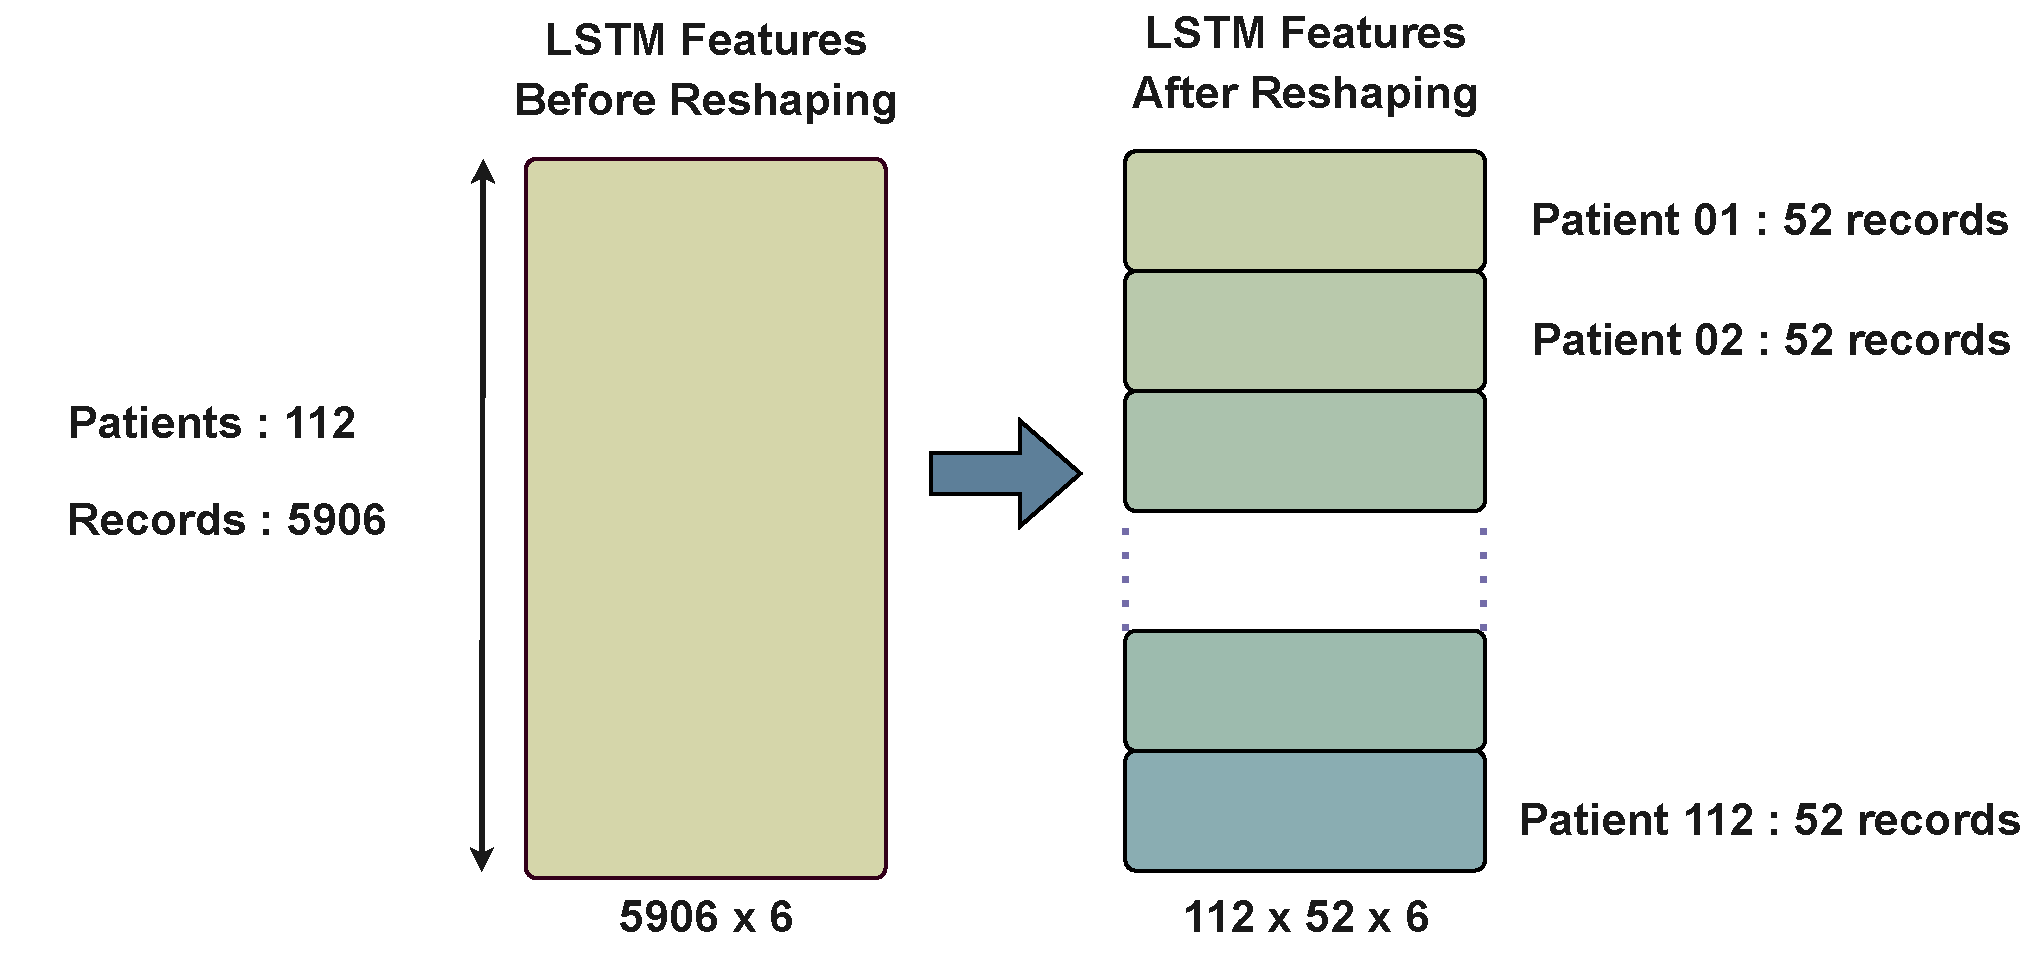
\includegraphics[width=0.7\linewidth]{images/dataReshaping.pdf}
    \caption{\textit{Data reshaping}}
    \label{fig:figure5}
    \vspace{-10pt}
\end{figure}


\subsubsection{Decision tree model}

In the medical domain, the clinical practice involves continuous decision-making, where optimal decision-making strives to maximize effectiveness and minimize loss \cite{b18}. Clinical decision analysis (CDA) highlights the significant role of decision trees in this process \cite{b19}. Among the five methodologies employed for decision-making, designing a decision tree is considered one \cite{b20}. Owing to their reliability, effectiveness, and high accuracy in decision-making, decision trees are widely utilized in various medical decision-making studies \cite{b21}. These factors led us to select the decision tree as the model to handle non-time-series data, including the \gls{lstm} outcome. The \gls{lstm} model is designed to generate a risk score based on time-series data acquired within a time window of up to 52 hours.

\subsubsection{Latent vector space}

Latent vector space is employed in machine learning to analyze data that can be mapped to a latent space where similar data points are in close proximity. In simpler terms, it can be described as a representation of compressed data. This latent space representation retains all the essential information required to represent the original data points, thereby facilitating data analysis. Latent space representations are utilized to transform more complex forms of raw data, such as images and videos, into simpler representations, a concept implemented in Representation Learning.

In the context of the \gls{lstm} model, the latent vector space serves as an input parameter for the decision tree model. The decision tree inputs are a combination of non-time-series data, including demographic information, lab results, triage score, Glasgow Coma Scale (GCS) values, and patient history, as well as the latent output of the \gls{lstm} model (Fig \ref{fig:figure6}). This approach allows for a more comprehensive analysis by integrating both time-series and non-time-series data, enhancing the model's decision-making capabilities.

\begin{figure}[hbt!]
    \centering
    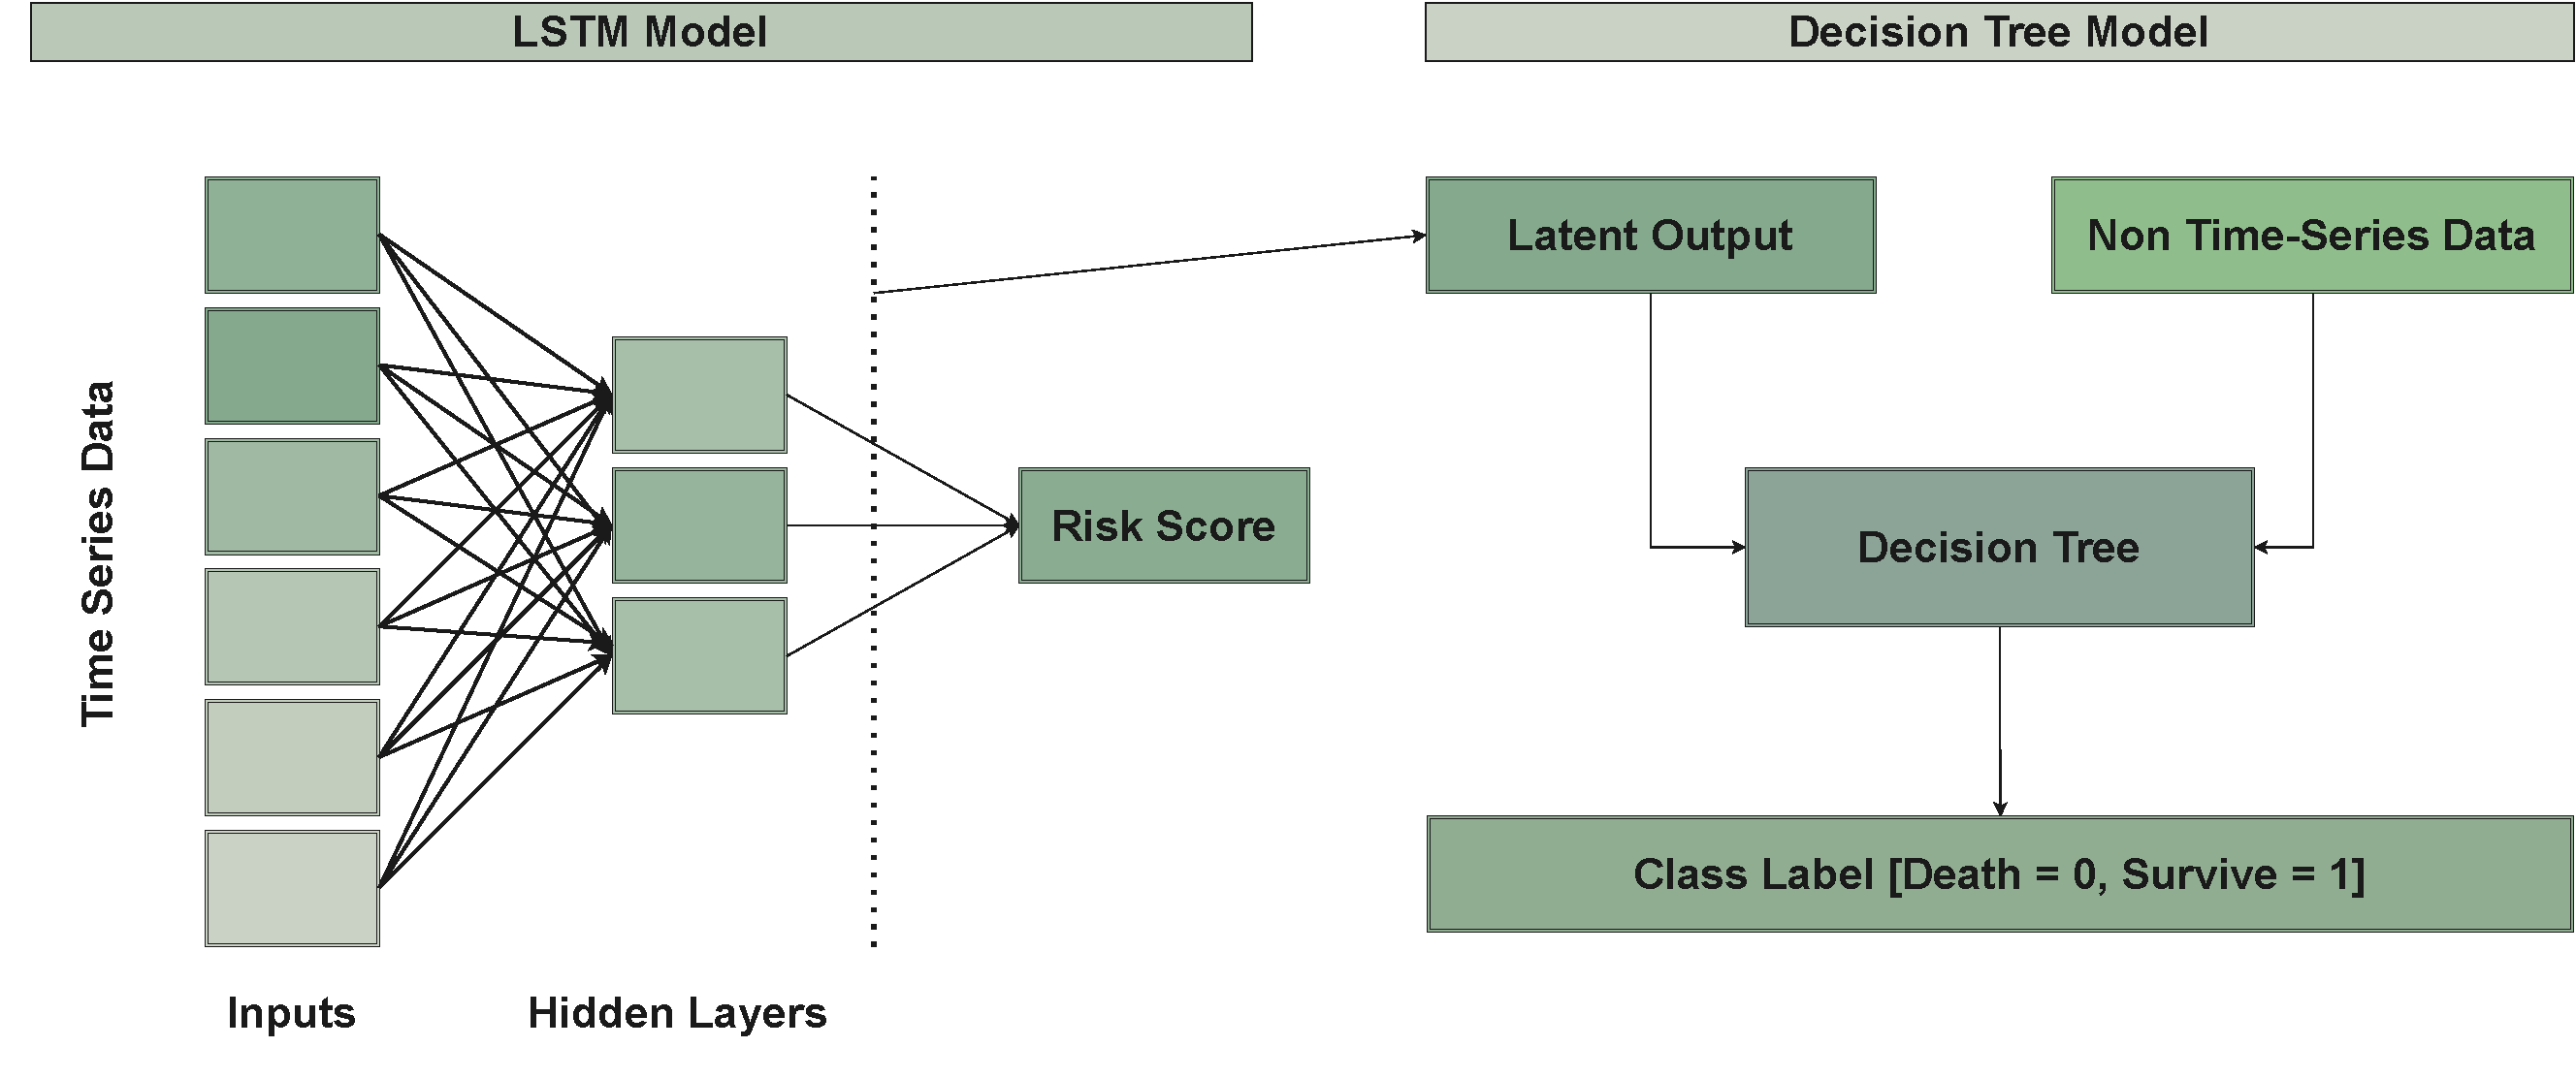
\includegraphics[width=\linewidth]{images/modelArchitecture.pdf}
    \caption{\textit{Model architecture}}
    \label{fig:figure6}
    \vspace{-10pt}
\end{figure}

\subsubsection{Dealing with Data Imbalance Problem}
Class imbalance is a common challenge in real-world data, particularly in medical fields, making it difficult to optimize machine learning algorithm performance. In this study, there were 93 majority-class (survived) and 19 minority-class (dead) patients, yielding a 1:5 ratio.

To address the class imbalance, Synthetic Minority Over-sampling Technique (SMOTE) was used first to over-sample the minority class, generating synthetic data and achieving a 1:1 class ratio. But as was recently demonstrated by Van den Goorbergh, SMOTE does not improve discrimination but does lead to models with strong miscalibration \cite{a23} we moved forward with the SDV to address the data imbalance problem.  

%%%%%%%%%%%%%%%%%%%%%%%%%%%%%%%%%%%%%%%%%%
\section{Results}
In this result section, we present the results of a series of comprehensive experiments conducted to assess the performance of the Deep Learning Cardiac Arrest Prediction Model. To enhance the robustness of our experiments, we incorporated SDV to generate synthetic data, permitting us to thoroughly assess the predictive capabilities of the model.
(Table \ref{tbl:experiments_table})
\begin{table}[hbt!]
\centering
\caption{Experiments performed by incorporating synthetic data to evaluate the results of the combined model. RS = Real Survived, RD = Real Dead, SS = Synthetic Survived, SD = Synthetic Dead. The survived: dead ratio of the patient was maintained at 1:1.}
\begin{tabular}{|c|c|c|c|c|c|}
\hline
Experiment No & RS & RD & SS & SD  & Accuracy \\ \hline
01            & 74 & 15 & -  & -   & 0.954    \\ \hline
02            & 74 & 15 & -  & 59  & 0.954    \\ \hline
03            & -  & -  & 74 & 74  & 0.964    \\ \hline
04            & 74 & 15 & 74 & 133 & 0.967    \\ \hline
\end{tabular}
\label{tbl:experiments_table}
\end{table}

After executing the designed experiments we were able to achieve peak accuracy through experiment 4 where the experiment encompassed a data set of 296 patient records. Hyperparameters were optimized according to the (Table \ref{tbl:table_1})

\begin{table}[hbt!]
\caption{Hyperparameter values}
\begin{center}
\resizebox{\columnwidth}{!}{
\begin{tabular}{|c|c|c|c|c|}
\hline
No of Epochs & Learning Rate & Batch Size & LSTM Nodes & Optimizer \\ \hline
100          & 0.001         & 10         & 2          & Adam      \\ \hline
\end{tabular}
}
\label{tab1}
\end{center}
\vspace{-20pt}
\label{tbl:table_1}
\end{table}

Creatinine levels were the most critical predictor, followed by sodium and blood urea levels. Studies suggest that these markers relate to renal function, which is linked to cardiovascular diseases \cite{b22}. Additionally, potassium levels, FHIHD, and age played key roles in classifying cardiac patients, supporting the association between cardiovascular diseases and decreased potassium levels \cite{b23}.

FHIHD is recognized as a well-established risk factor for cardiovascular diseases \cite{b24}. In the study's findings, the risk factor FHIHD emerged as one of the most reliable predictive features for cardiac arrests. (Fig \ref{fig:figure7}) displays the probabilistic prediction window for six randomly selected patients (three from each of the two classes).
The \gls{lstm} model itself was proficient in providing predictions from the time of admission up to 52 hours later. In other words, the model's prediction window spanned 52 hours. The model demonstrated a prediction accuracy of 96\% with a confidence interval of 95.01\% to 95.85\%.

%\begin{figure}[hbt!]
    \centering
    \begin{subfigure}{0.45\linewidth}
        \centering
        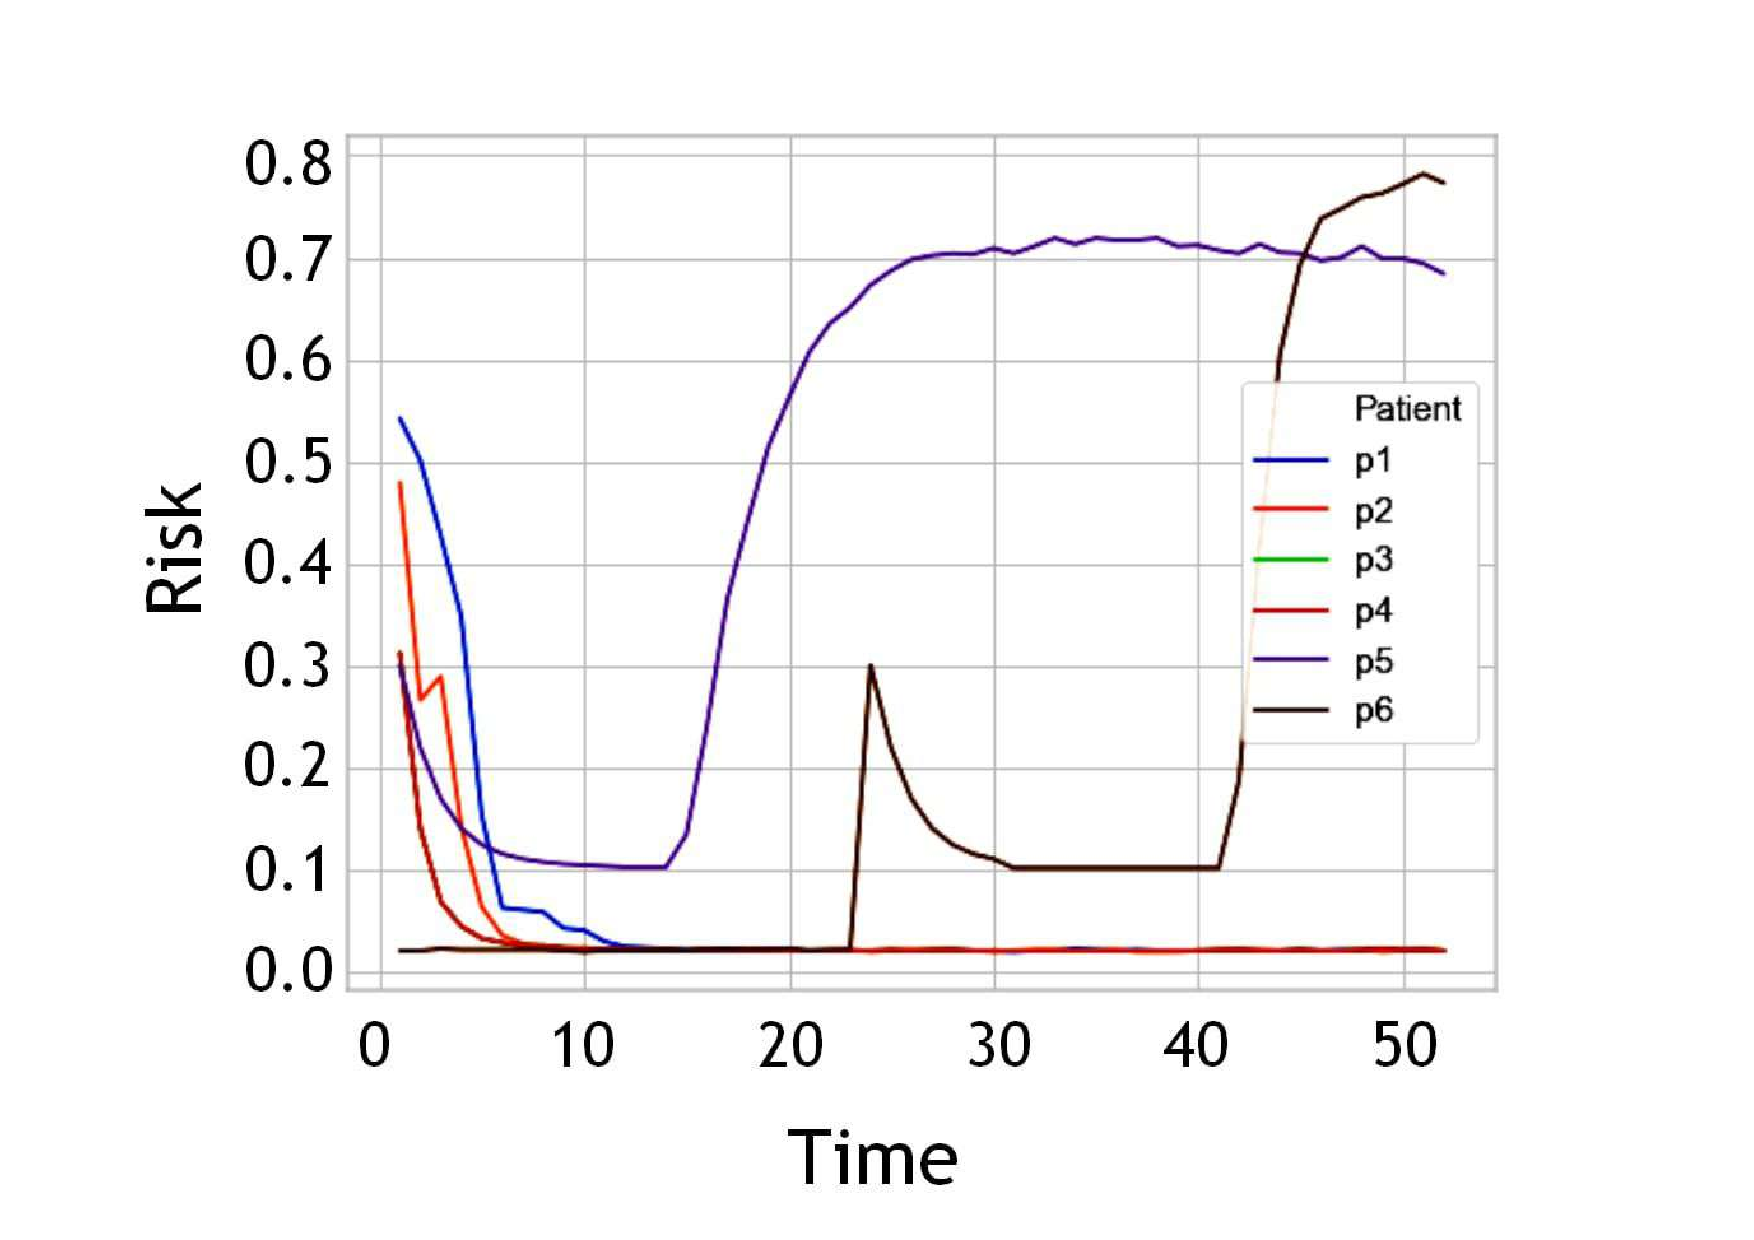
\includegraphics[width=\linewidth]{images/riskPrediction.pdf}
        \caption{\textit{Prediction of the risk score with 52 hours}}
        \label{fig:figure7}
    \end{subfigure}
    \hfill
    \begin{subfigure}{0.45\linewidth}
        \centering
        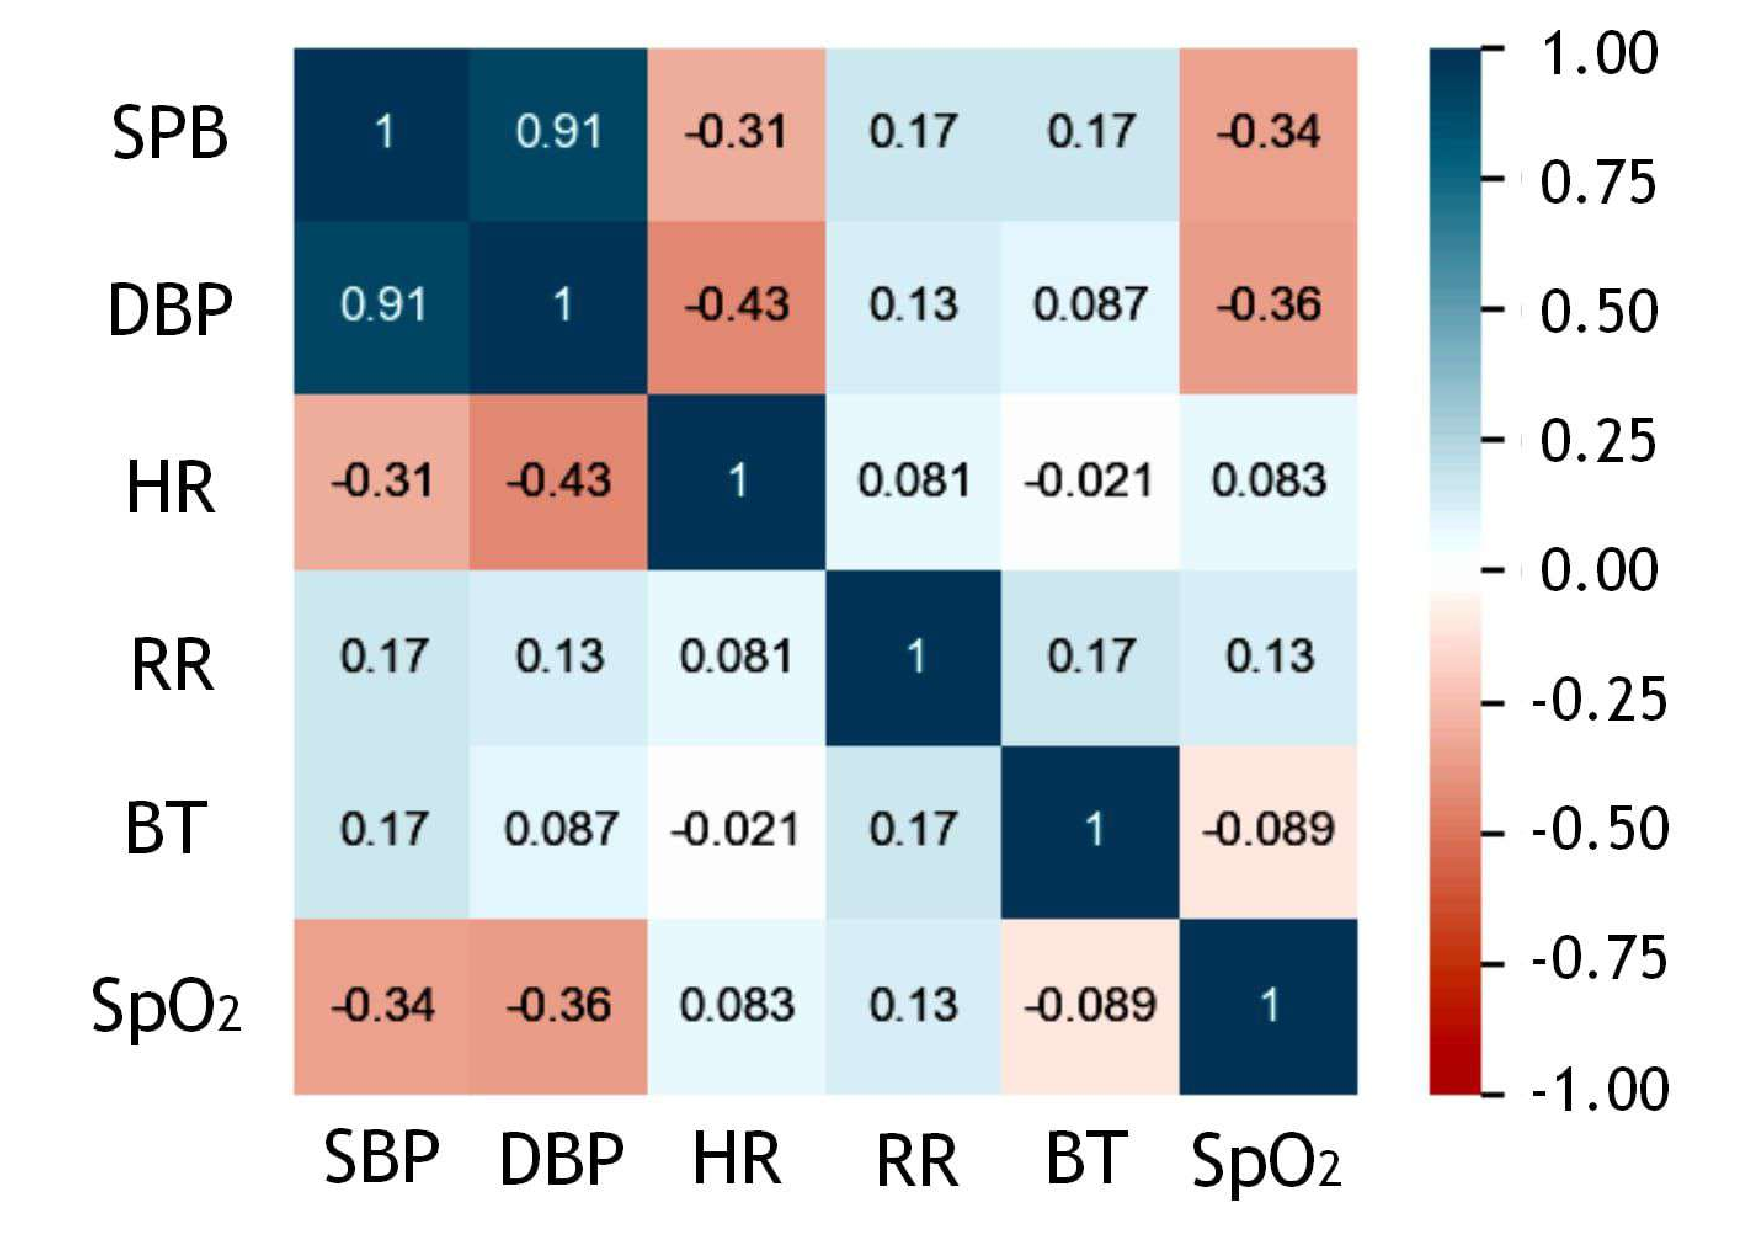
\includegraphics[width=\linewidth]{images/correlations.pdf}
        \caption{\textit{Correlation heatmap between time-series inputs}}
        \label{fig:figure8}
    \end{subfigure}
    \caption{Risk prediction and correlation heatmap}
    \label{fig:figure7_8}
\end{figure}

% Start from here
\begin{figure}[hbt!]
    \centering
    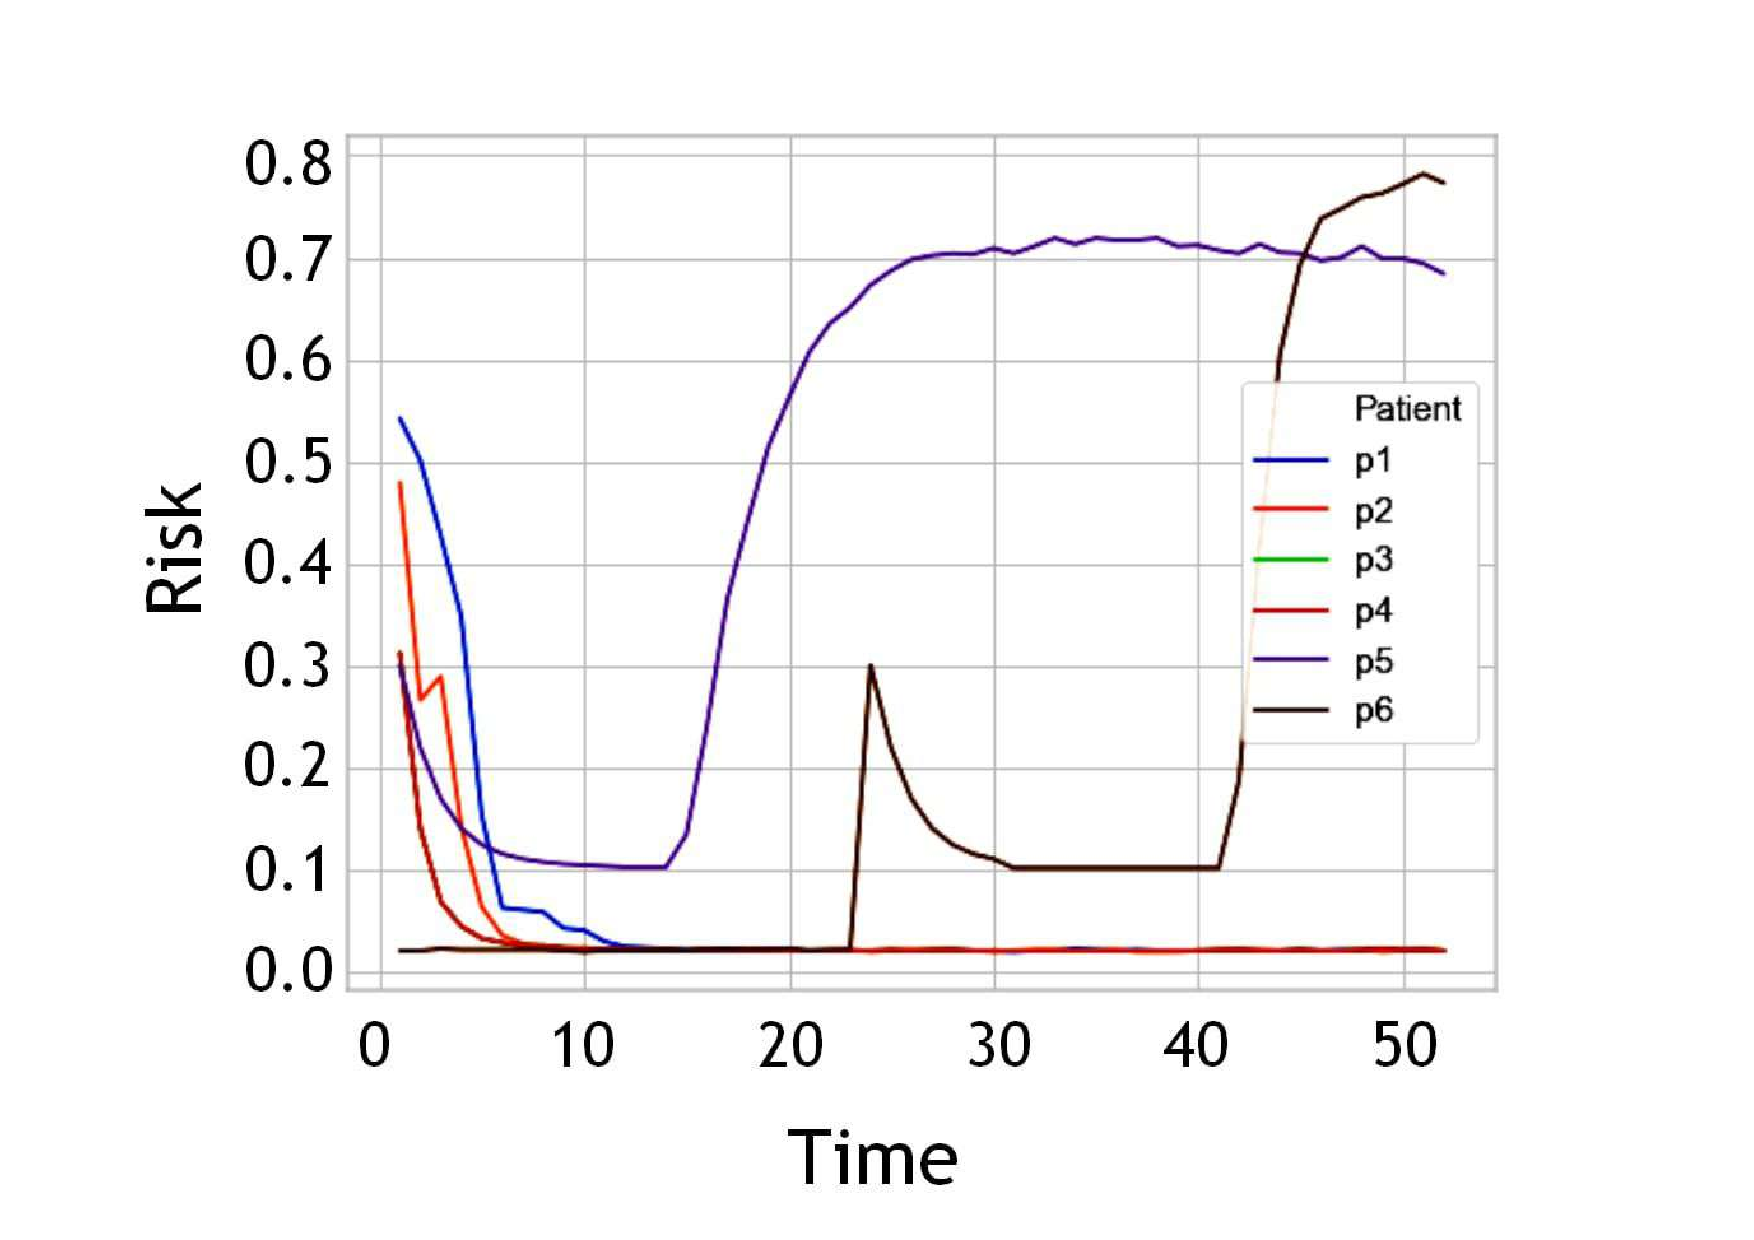
\includegraphics[width=0.75\linewidth]{images/riskPrediction.pdf}
    \caption{\textit{Prediction of the risk score with 52 hours}}
    \label{fig:figure7}
    \vspace{-10pt}
\end{figure}

\subsection{Comparison with existing models}
We assessed the performance of the developed Deep Learning Cardiac Arrest Prediction Model (DLCAPM) by comparing it with well-established machine learning algorithms, such as Logistic Regression, Random Forest, Naïve Bayes, and Support Vector Machine (SVM). The evaluation was carried out using all the features incorporated in the DLCAPM model. Table \ref{tbl:table_2} presents the performance metrics, including Accuracy, Sensitivity, Specificity, Positive Predictive Value (PPV), Negative Predictive Value (NPV), and F-Score, for each of the compared models. The results demonstrate that the \gls{lstm} component of the DLCAPM model exhibits superior performance in comparison to the selected models.
\begin{table}[!t]
\caption{Performance comparison with existing machine learning models (LSTM \& Decision Tree are the two models of Deep Learning Cardiac Arrest Prediction Model[DLCAPM])}
\resizebox{\columnwidth}{!}{%
\begin{tabular}{|c|c|c|c|c|c|c|}
\hline
\textbf{Model }           & \textbf{Accuracy} & \textbf{Sensitivity} & \textbf{Specificity} & \textbf{PPV}  & \textbf{NPV}  & \textbf{F-Score} \\ 
\hline
\textbf{LSTM} &
  \begin{tabular}[c]{@{}c@{}}\textbf{0.96}\end{tabular} &
  \begin{tabular}[c]{@{}c@{}}\textbf{0.95} \end{tabular} &
  \textbf{0.93} &
  \textbf{0.98} &
  \textbf{0.81} &
  \textbf{0.86} \\ \hline
\textbf{Decision Tree} &
  \begin{tabular}[c]{@{}c@{}} \textbf{0.76}\end{tabular} &
  \begin{tabular}[c]{@{}c@{}} \textbf{0.69}\end{tabular} &
  \textbf{0.81} &
  \textbf{0.72} &
  \textbf{0.79} &
  \textbf{0.80} \\ \hline
SVM                 & 0.89     & 0.84        & 0.82        & 0.81 & 0.82 & 0.844   \\ \hline
Logistic Regression & 0.88     & 0.93        & 0.81        & 0.92 & 0.81 & 0.87    \\ \hline
Random Forest       & 0.88     & 0.89        & 0.90        & 0.87 & 0.81 & 0.91    \\ \hline
Naive Bayes         & 0.85     & 0.89        & 0.80        & 0.82 & 0.88 & 0.91    \\ \hline
\end{tabular}%
}
\label{tbl:table_2}
\vspace{-10pt}
\end{table}

\subsection{Correlation analysis}

Correlation analysis evaluates the relationships among model input features. Pearson's and Spearman's coefficients are commonly used; the former is for normally distributed variables and the latter for skewed or ordinal variables. A coefficient near ±1 indicates a strong correlation, either positive or negative \cite{b25}. In this study, Spearman's rank correlation was used due to Gaussian distribution, and Fig \ref{fig:figure8} shows the heatmap of correlation coefficients. A high positive correlation exists between Systolic and Diastolic Blood Pressure.

\begin{figure}[hbt!]
    \centering
    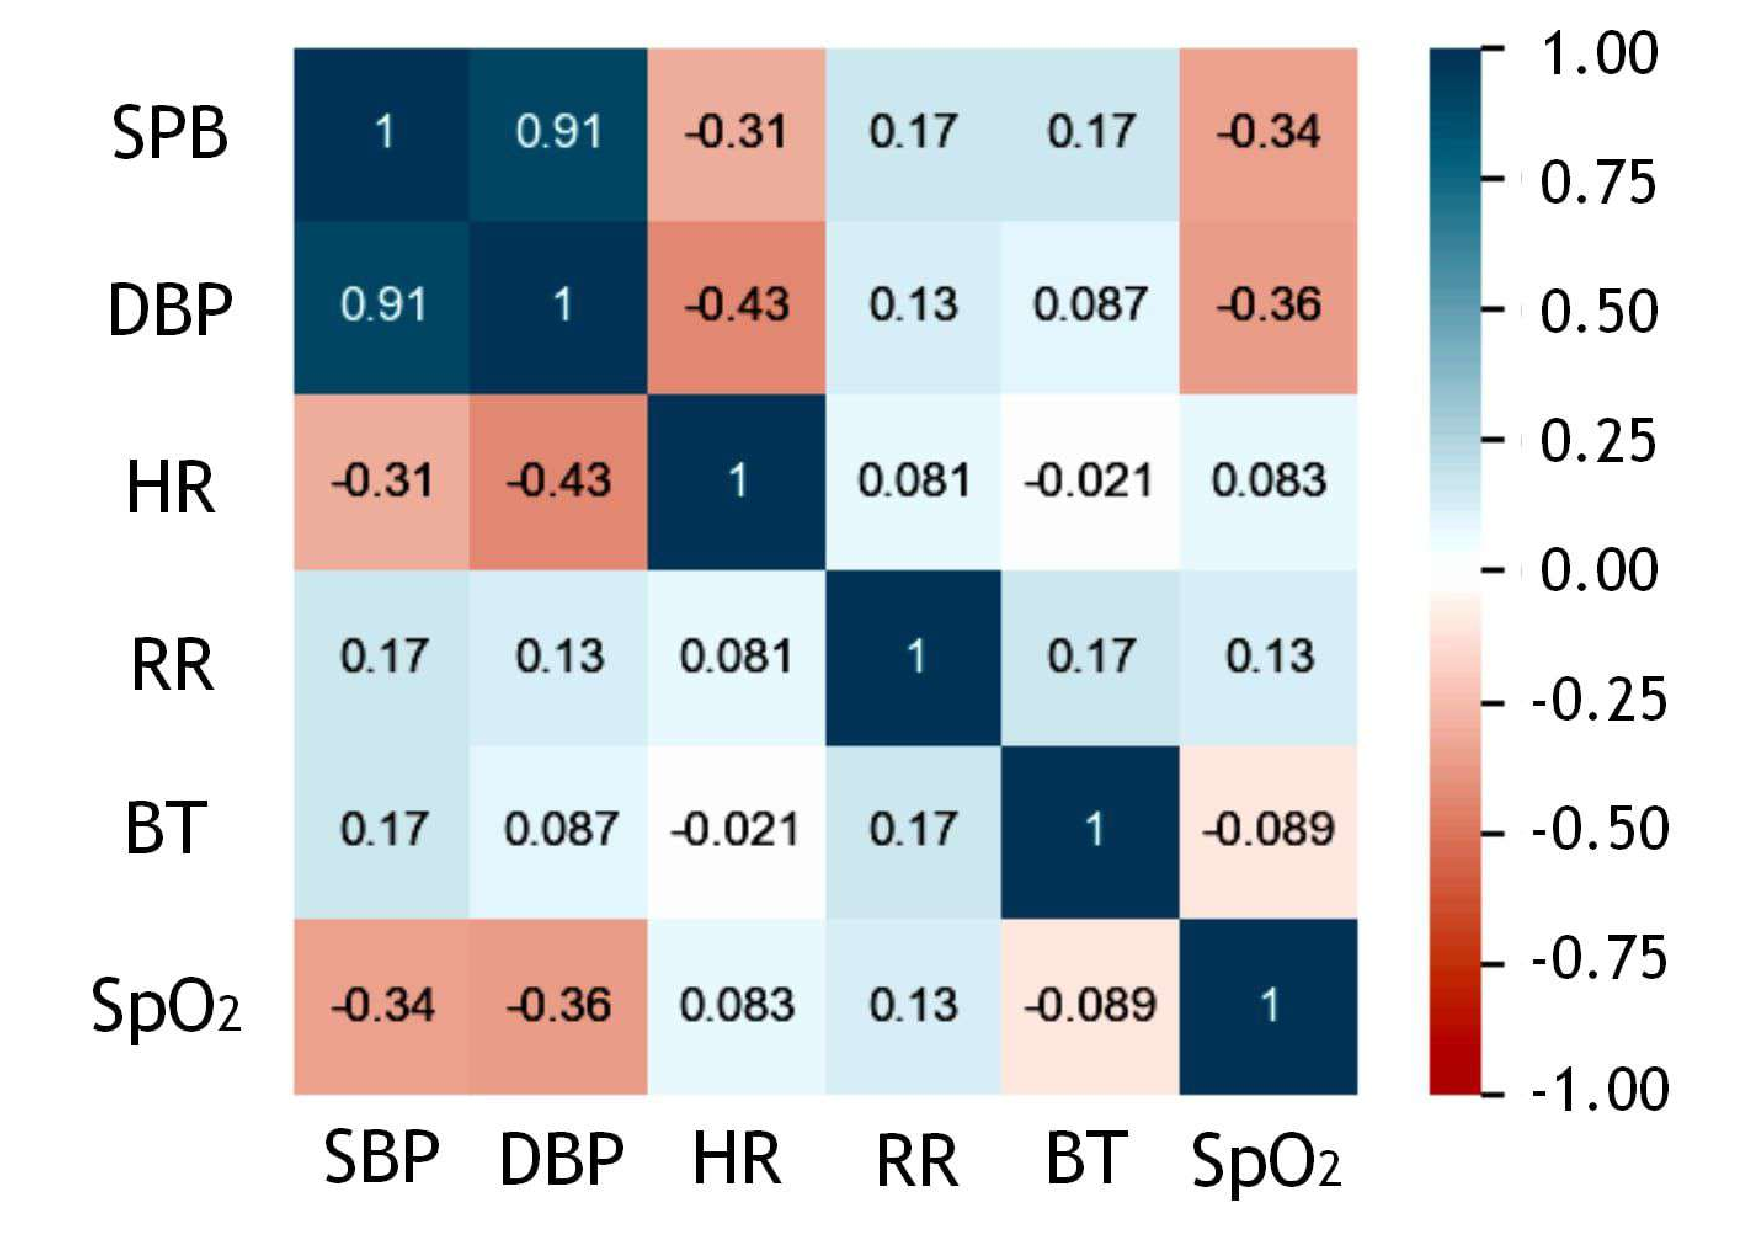
\includegraphics[width=0.75\linewidth]{images/correlations.pdf}
    \caption{\textit{Correlation heatmap between time-series inputs}}
    \label{fig:figure8}
    \vspace{-10pt}
\end{figure}

\subsection{Characteristics of the study population}

In the cohort study, patient data were analyzed to assess the observed characteristics of the study population, as shown in Table \ref{tbl:table_3}. From these observations, we can infer that males may have a higher susceptibility to cardiovascular diseases and cardiac arrests. This study also examined the impact of various risk factors that could potentially contribute to the development of \glspl{cvd}. Among these risk factors, alcohol consumption, smoking, and a family history of ischemic heart disease (FHIHD) were identified as the most significant contributors. In the total population (comprising both males and females), 37\% of individuals reported having an FHIHD. Notably, none of the female patients were documented to consume alcohol or smoke. Among the male patients, 73\% (81 patients) were found to engage in at least one of these behaviors, with 69\% (55 patients) consuming alcohol, 63\% (51 patients) smoking, and 26\% (21 patients) engaging in both alcohol consumption and smoking.

\begin{table}[!t]
\caption{Characteristics of the study population}
\begin{center}
\resizebox{\columnwidth}{!}{%
\begin{tabular}{|c|l|}
\hline
\textbf{Characteristic}             & \multicolumn{1}{c|}{\textbf{Data}}             \\ \hline
Study period                        & 13th of August 2018 - 6th of February 2020     \\ \hline
Hospital                            & Teaching Hospital Karapitiya, Galle, Sri Lanka \\ \hline
Total patients, n                   & 112                                            \\ \hline
Input vectors, n                    & 19                                             \\ \hline
Age group                           & 59 – 76years                                   \\ \hline
Male, n (\%)                        & 73\%                                           \\ \hline
Symptoms before admission &
  \begin{tabular}[c]{@{}l@{}}Chest pain on the left side (1/2 hour before the admission), \\ Tightening of the chest, Vomiting, Sweating, Nausea, Cough, Fever\end{tabular} \\ \hline
Patients with FHIHD, n (\%)         & 37\%                                           \\ \hline
Consume alcohol, Male n (\%)        & 69\%                                           \\ \hline
Smoking, Male n (\%)                & 63\%                                           \\ \hline
Smoking \& use alcohol, Male n (\%) & 26\%                                           \\ \hline
\end{tabular}%
}
\end{center}
\label{tbl:table_3}
\vspace{-10pt}
\end{table}
%%%%%%%%%%%%%%%%%%%%%%%%%%%%%%%%%%%%%%%%%%
\section{Discussion}

The performance of the model was assessed using two optimization algorithms, 'Adam' and 'Admax'. Multiple iterations were performed, altering hyperparameter combinations to identify the four most optimal configurations, which yielded the highest accuracy. Table \ref{tbl:table_4} presents the evaluation metrics for each of these four selected runs. Among these experiments, the best results were achieved in experiment number 04 for training the model.

\begin{table}[!t]
\caption{Performance of the model for four experimental data sets. Here, we tested the LSTM and the Decision tree model separately}
\begin{center}
\resizebox{\columnwidth}{!}{%
{\tiny
\begin{tabular}{|c|cccc|cccc|}
\hline
\multirow{3}{*}{\textbf{Metric}} & \multicolumn{4}{c|}{\textbf{LSTM}}     & \multicolumn{4}{c|}{\textbf{Decision Tree}}    \\ \cline{2-9} 
                                 & \multicolumn{4}{c|}{Experiment number} & \multicolumn{4}{c|}{Experiment number} \\ \cline{2-9} 
 &
  \multicolumn{1}{c|}{01} &
  \multicolumn{1}{c|}{02} &
  \multicolumn{1}{c|}{03} &
  \textbf{04} &
  \multicolumn{1}{c|}{01} &
  \multicolumn{1}{c|}{02} &
  \multicolumn{1}{c|}{03} &
  \textbf{04} \\ \hline
Accuracy &
  \multicolumn{1}{c|}{0.93} &
  \multicolumn{1}{c|}{0.85} &
  \multicolumn{1}{c|}{0.94} &
  \textbf{0.96} &
  \multicolumn{1}{c|}{0.80} &
  \multicolumn{1}{c|}{0.83} &
  \multicolumn{1}{c|}{0.80} &
  \textbf{0.76} \\ \hline
Precision &
  \multicolumn{1}{c|}{1.0} &
  \multicolumn{1}{c|}{1.0} &
  \multicolumn{1}{c|}{1.0} &
  \textbf{1.0} &
  \multicolumn{1}{c|}{1.0} &
  \multicolumn{1}{c|}{1.0} &
  \multicolumn{1}{c|}{1.0} &
  \textbf{1.0} \\ \hline
Recall &
  \multicolumn{1}{c|}{1.0} &
  \multicolumn{1}{c|}{1.0} &
  \multicolumn{1}{c|}{1.0} &
  \textbf{1.0} &
  \multicolumn{1}{c|}{1.0} &
  \multicolumn{1}{c|}{1.0} &
  \multicolumn{1}{c|}{1.0} &
  \textbf{10} \\ \hline
F-Score &
  \multicolumn{1}{c|}{0.81} &
  \multicolumn{1}{c|}{0.86} &
  \multicolumn{1}{c|}{0.81} &
  \textbf{0.86} &
  \multicolumn{1}{c|}{0.82} &
  \multicolumn{1}{c|}{0.85} &
  \multicolumn{1}{c|}{0.82} &
  \textbf{0.80} \\ \hline
AUC score &
  \multicolumn{1}{c|}{0.97} &
  \multicolumn{1}{c|}{0.95} &
  \multicolumn{1}{c|}{0.97} &
  \textbf{0.98} &
  \multicolumn{1}{c|}{0.79} &
  \multicolumn{1}{c|}{0.83} &
  \multicolumn{1}{c|}{0.79} &
  \textbf{0.75} \\ \hline
\end{tabular}%
}
}
\end{center}
\label{tbl:table_4}
\vspace{-10pt}
\end{table}

Table \ref{tbl:table_5} shows the sensitivity, specificity, Positive Predictive Value (PPV), Negative Predictive Value (NPV), and accuracy measures for the outperformed \gls{lstm} model and decision tree model in experiment number 04, respectively.

\begin{table}[!t]
\captionsetup{justification=raggedright,singlelinecheck=false,font={small}}
\caption{Evaluation metrics of LSTM and Decision Tree models of the Deep Learning Cardiac Arrest Prediction Model}
\label{table:models}
    \centering
    \resizebox{\columnwidth}{!}{%
    \begin{tabular}{|c|cc|cc|}
    \hline
    \multirow{2}{*}{\textbf{Statistic}} & \multicolumn{2}{c|}{\textbf{Value}} & \multicolumn{2}{c|}{\textbf{95\% CI}} \\ \cline{2-5} 
    & \multicolumn{1}{c|}{LSTM Model} & Decision Tree Model & \multicolumn{1}{c|}{LSTM Model} & Decision Tree Model \\ \hline
    Sensitivity & \multicolumn{1}{c|}{95.83\%} & 69.57\% & \multicolumn{1}{c|}{95.37\% to 96.25\%} & 47.08\% to 86.79\% \\ \hline
    Specificity & \multicolumn{1}{c|}{93.42\%} & 81.82\% & \multicolumn{1}{c|}{92.07\% to 94.61\%} & 64.54\% to 93.02\% \\ \hline
    Positive Predictive Value  & \multicolumn{1}{c|}{98.71\%} & 72.73\% & \multicolumn{1}{c|}{98.44\% to 98.93\%} & 55.19\% to 85.24\% \\ \hline
    \begin{tabular}[c]{@{}c@{}}Negative Predictive\\ Value\end{tabular} & \multicolumn{1}{c|}{81.04\%} & 79.41\% & \multicolumn{1}{c|}{79.37\% to 
    82.60\%} & 67.07\% to 87.96\% \\ \hline
    \end{tabular}%
    }
    \label{tbl:table_5}
    \vspace{-10pt}
\end{table}

The ROC curve is a graphical representation that demonstrates the diagnostic ability of binary classifiers by plotting sensitivity against specificity. A better-performing classifier will have a curve closer to the top-left corner. To compare classifiers' performance, a common approach is to calculate the area under the ROC curve. Figure \ref{fig:figure9} presents the ROC curve for the \gls{lstm} model.

However, visual interpretations and comparisons of ROC curves can be misleading for imbalanced datasets. To address this issue, precision-recall curves are utilized. Figure \ref{fig:figure10} illustrates the precision-recall curve for the LSTM model, and the supplementary figure shows the curve for the decision tree classifier model.

\begin{figure}[hbt!]
    \centering
    \begin{subfigure}{0.45\linewidth}
        \centering
        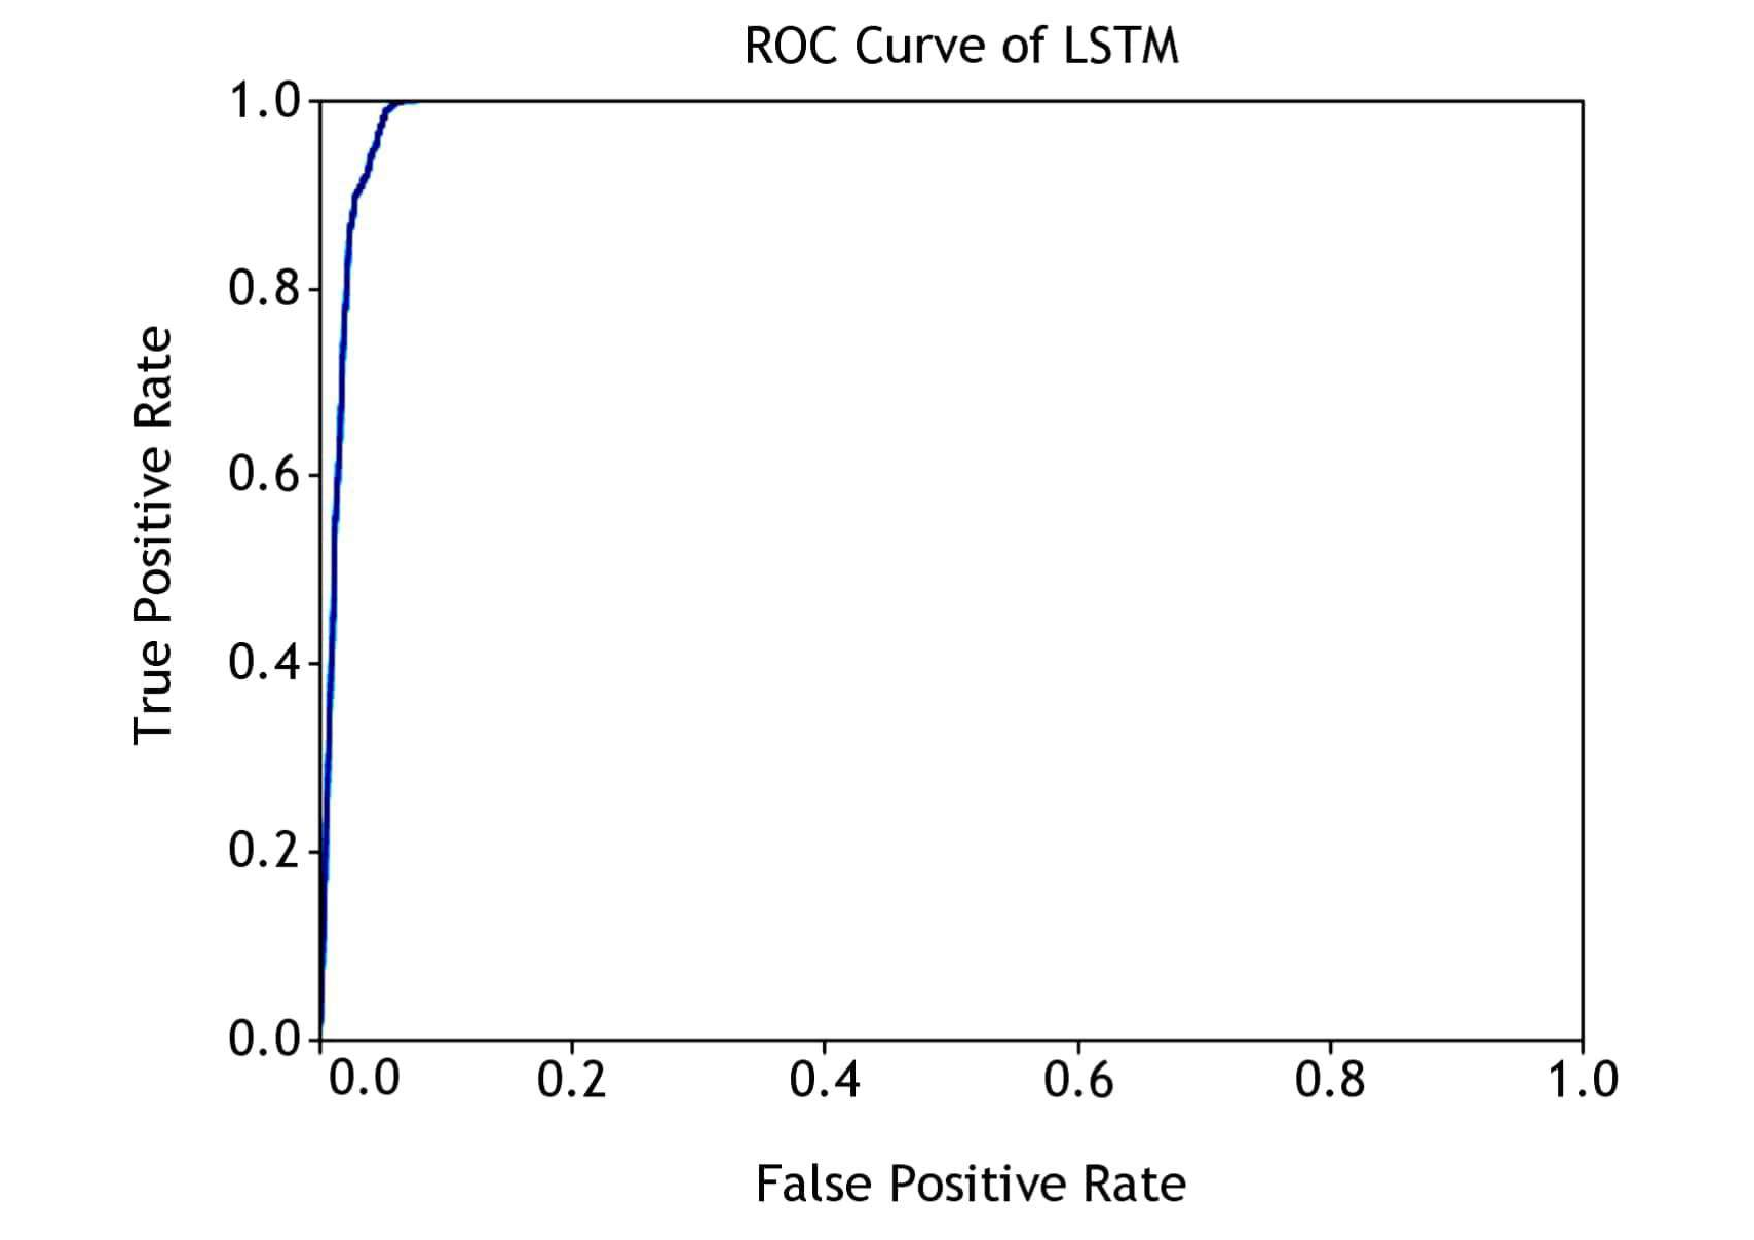
\includegraphics[width=\linewidth]{images/ROC_LSTM.pdf}
        \caption{\textit{ROC curve }}
        \label{fig:figure9}
    \end{subfigure}
    \hfill
    \begin{subfigure}{0.45\linewidth}
        \centering
        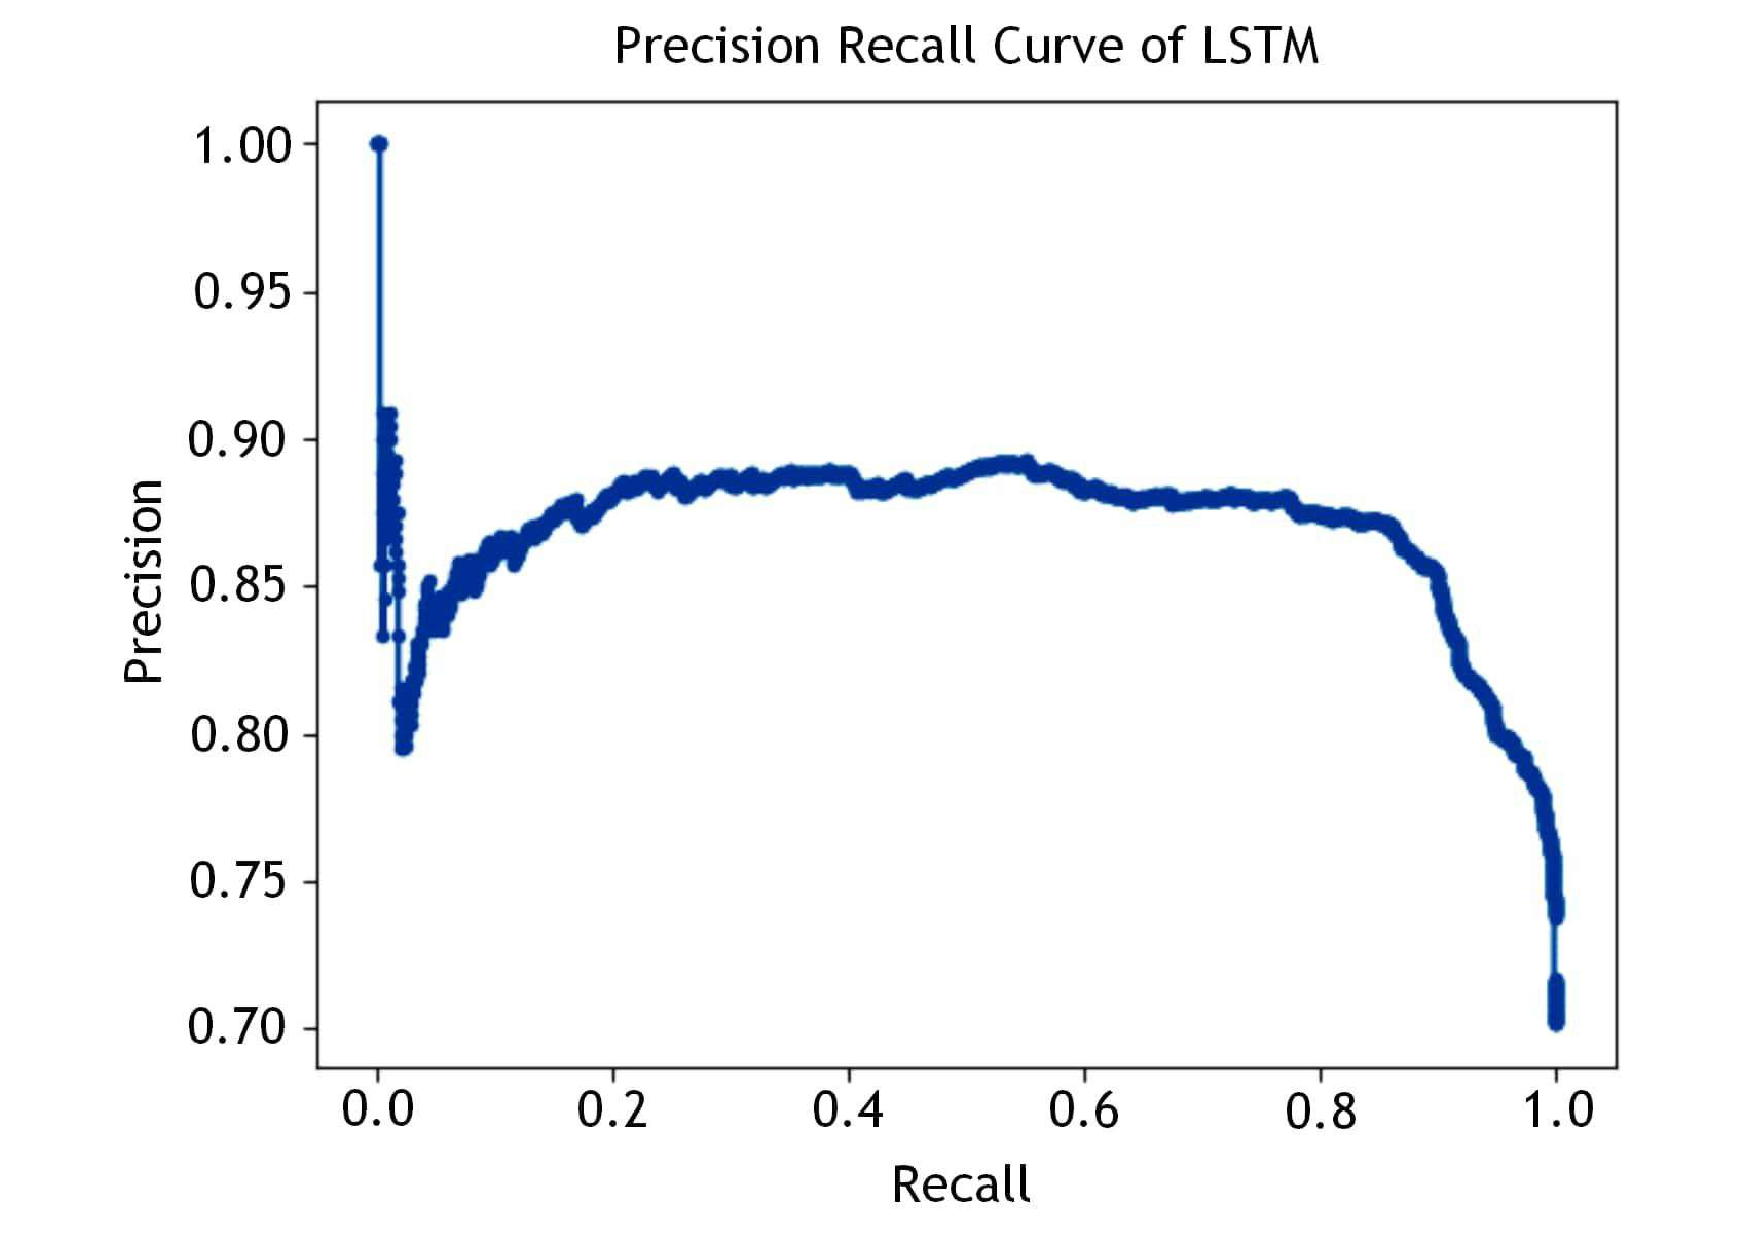
\includegraphics[width=\linewidth]{images/precisionRecallLSTM.pdf}
        \caption{\textit{Precision-Recall curve}}
        \label{fig:figure10}
    \end{subfigure}
    \caption{ROC curve and Precision-Recall curve of LSTM model}
    \label{fig:figure9_10}
    \vspace{-10pt}
\end{figure}


The confusion matrix, crucial for statistical classifications in machine learning, is a table describing a classification model's performance and identifying class confusion. Figure \ref{fig:figure11} and Figure \ref{fig:figure12} display the confusion matrices for the \gls{lstm} and decision tree models, respectively.


\begin{figure}[hbt!]
    \centering
    \begin{subfigure}[b]{0.45\linewidth}
        \centering
        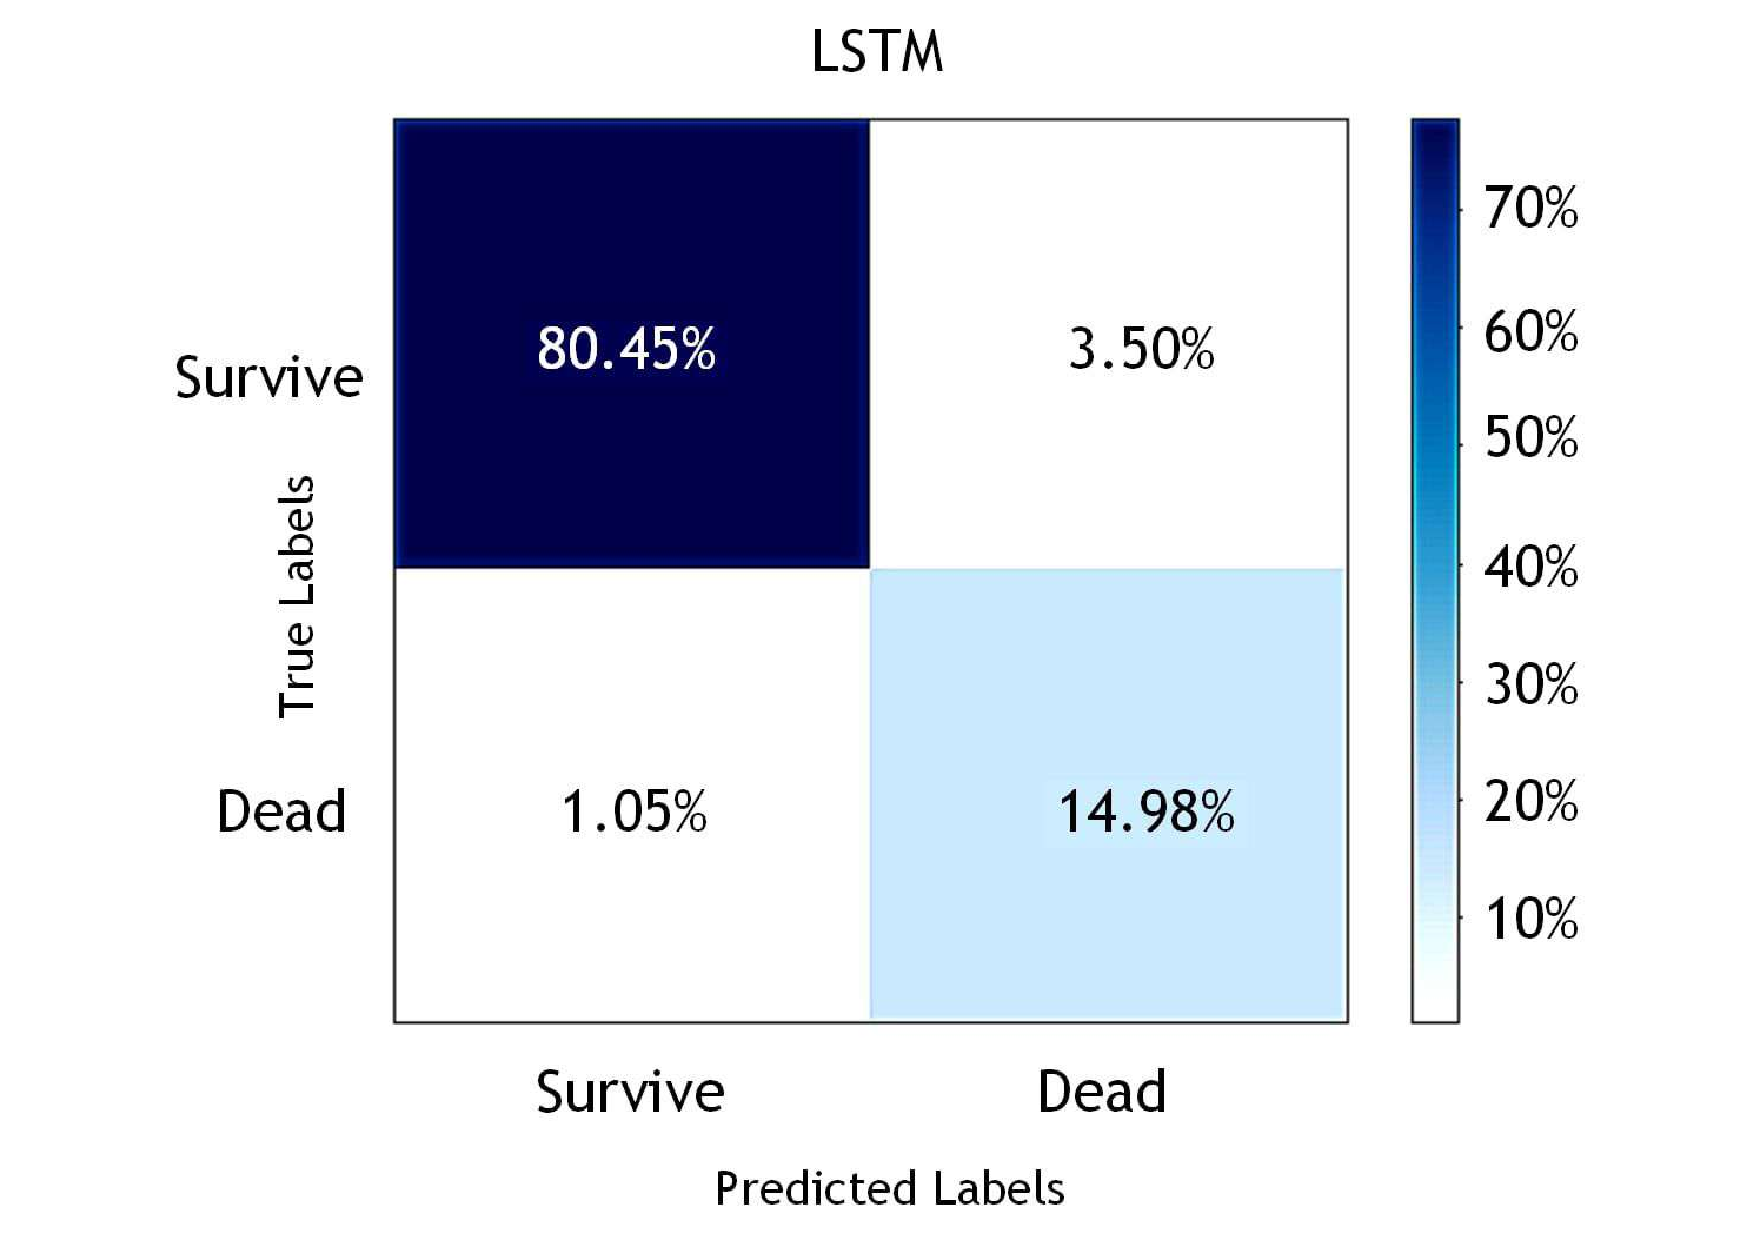
\includegraphics[width=\linewidth, height=\linewidth]{images/LSTM_Con.pdf}
        \caption{\textit{Confusion matrix for LSTM model}}
        \label{fig:figure11}
    \end{subfigure}
    \hfill
    \begin{subfigure}[b]{0.45\linewidth}
        \centering
        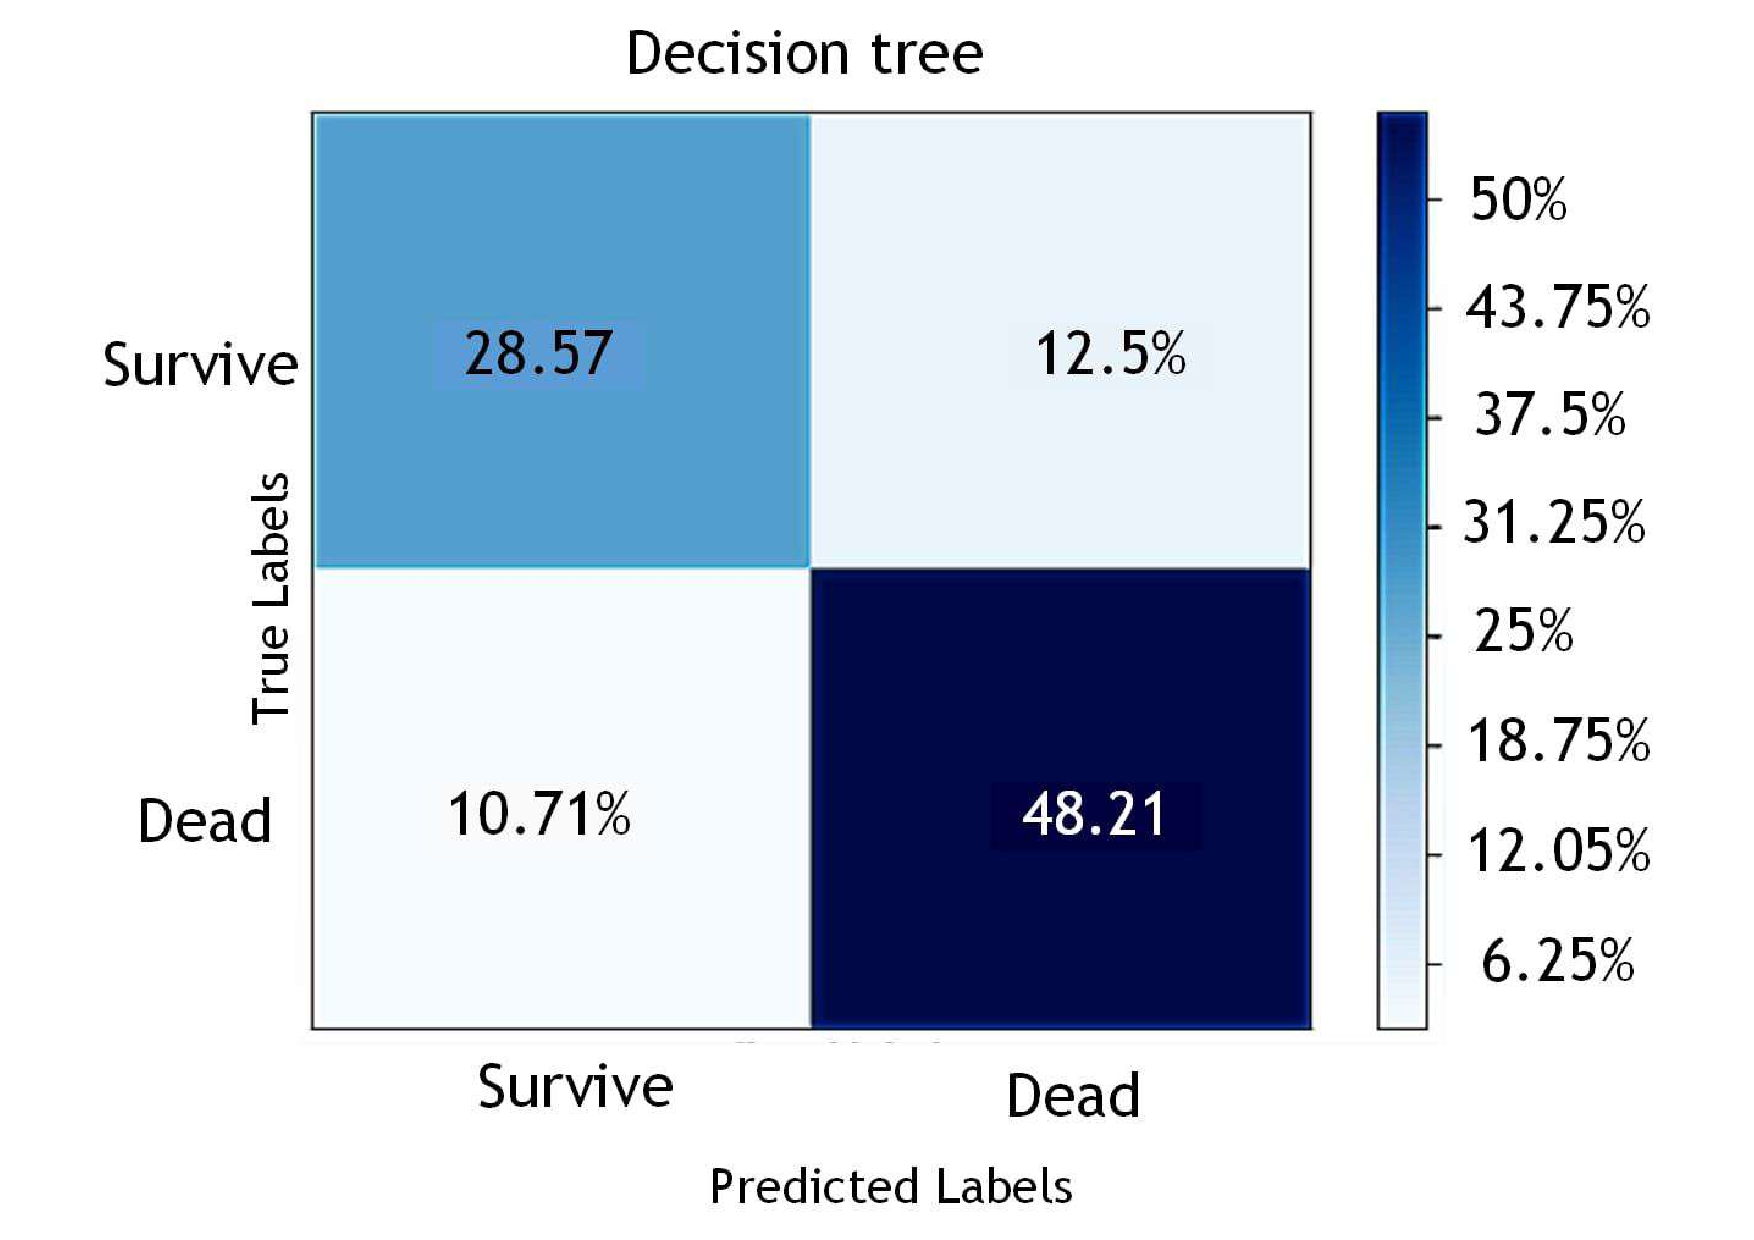
\includegraphics[width=\linewidth, height=\linewidth]{images/DecisionTree_Con.pdf}
        \caption{\textit{Confusion matrix for the decision tree model}}
        \label{fig:figure12}
    \end{subfigure}
    \caption{\textit{Confusion matrices for (a) LSTM model and (b) decision tree model}}
    \label{fig:confusion_matrices}
    \vspace{-10pt}
\end{figure}

\subsubsection{Comparison with existing EWS}
 
DLCAPM was evaluated against existing cardiac arrest early warning scores, including Modified Early Warning Score (MEWS), Cardiac Arrest Risk Triage Score (CART), and National Early Warning Score (NEWS), based on research by \cite{b26, b27}. MDCALC calculator \cite{b28, b29, b30} was used to calculate risk scores for CART, MEWS, and NEWS using collected data (RR, SpO2, BT, SBP, DBP, HR, Age, Triage Score). Table \ref{tbl:table_6} displays the performance of each score.

\begin{table}[htbp]
\caption{Performance comparison of DLCAPM(Deep Learning Cardiac Arrest Prediction Model: Combination of LSTM and Decision Tree) against CART(Cardiac Arrest Risk Triage Score), MEWS(Modified Early Warning Score) and NEWS(National Early Warning Score) models. Highlighted are the results of the DLCAPM. } 
\resizebox{\columnwidth}{!}{%
\begin{tabular}{|c|c|c|c|c|c|c|}
\hline
\textbf{Model}  & \textbf{Accuracy} & \textbf{Sensitivity} & \textbf{Specificity} & \textbf{PPV}         & \textbf{NPV}         & \textbf{F-Score}
\\ \hline
\textbf{LSTM} & \textbf{0.96} & \textbf{0.95}  & \textbf{0.93} & \textbf{0.98}  & \textbf{0.81} & \textbf{0.86}  \\ \hline
\textbf{Decision Tree} & \textbf{0.76} & \textbf{0.69} & \textbf{0.81} & \textbf{0.72} & \textbf{0.79} & \textbf{0.80} \\ \hline
CART & 0.60 & 0.50 & 0.75 & 0.75 & 0.75 & 0.60 \\ \hline
MEWS & 0.80 & 0.93 & 0.40 & 0.82 & 0.4  & 0.50 \\ \hline
NEWS & 0.80 & 0.84 & 0.66 & 0.94 & 0.66 & 0.66 \\ \hline
\end{tabular}%
}
\label{tbl:table_6}
\vspace{-10pt}
\end{table}

\subsubsection{Limitations}

The THK record room utilizes Microsoft Excel to store limited data from bedhead tickets, making it necessary to manually review each patient's record to obtain the required information for this study, which was time-consuming. The small sample size, potential patient heterogeneity, and focus on a specific patient population within a single hospital unit limit the research's generalizability, making it potentially inapplicable nationwide. These limitations stem from the legacy methods of maintaining patient data and difficulties in retrieval.

Due to limited resources, only 112 patient records were extracted, which prevented reaching the desired sample size for the model. To address this limitation, the Synthetic Data Vault Technique (SDV) was employed to increase the minority sample size. Furthermore, the study faced constraints due to the scarcity of local research on the development of cardiac arrest \glspl{ews} in Sri Lanka \cite{b8, b10}.

%%%%%%%%%%%%%%%%%%%%%%%%%%%%%%%%%%%%%%%%%%
\section{Conclusions}

An efficient deep-learning cardiac risk prediction model was developed using clinical features from THK cardiac patients' BHTs. This simple model uses accessible patient data, offering bedside support for healthcare workers and assisting decision-making. An open-access dataset was published to encourage further research.

Early and accurate predictions can aid in timely interventions and prevent cardiac events. Despite high accuracy, addressing data limitations could improve the model. Further research is needed to explore applicability in other healthcare settings and integration with existing patient monitoring tools for enhanced prediction.
%%%%%%%%%%%%%%%%%%%%%%%%%%%%%%%%%%%%%%%%%%

\authorcontributions{ L.R. Study concept and design; acquisition of data; analysis and interpretation of data; drafting of the manuscript; statistical analysis. S.V: Study concept and design;
Critical revision of the manuscript; Drafting of the manuscript.
V.T: Study concept and design; Critical revision of the manuscript; Drafting of the manuscript; Supervision. S.G: Study concept and design; Critical revision of the manuscript; Drafting of the manuscript; Supervision. All authors have read and agreed to the published version of the manuscript.
}
\funding{This research received no external funding}

\institutionalreview{The study was conducted in accordance with the Ethics Committee of Faculty of Medicine University of Ruhuna, Sri Lanka (protocol code 2019/P/063 and date of approval 27.11.2019).”}

\informedconsent{
Since this study was carried out as a retrospective study, obtaining informed consent from all subjects was not applicable.

}

\dataavailability{
The dataset used for all experiments is publicly available at \url{https://zenodo.org/record/7603772}
% We encourage all authors of articles published in MDPI journals to share their research data. In this section, please provide details regarding where data supporting reported results can be found, including links to publicly archived datasets analyzed or generated during the study. Where no new data were created, or where data is unavailable due to privacy or ethical re-strictions, a statement is still required. Suggested Data Availability Statements are available in section “MDPI Research Data Policies” at \url{https://www.mdpi.com/ethics}.
} 

\acknowledgments{
The authors express their gratitude for the support provided by Dr. Susitha Amarasinghe, Professor Sampath Gunawardena, Mrs. S.G.H. Uluwaduge, Mr. Bhashithe Abeysinghe, Dr. Samadhi Rajapaksha, and the Ethics Review Committee of the Faculty of Medicine, University of Ruhuna.

% In this section you can acknowledge any support given which is not covered by the author contribution or funding sections. This may include administrative and technical support, or donations in kind (e.g., materials used for experiments).
}

\conflictsofinterest{
The authors declare no conflict of interest.
% Declare conflicts of interest or state ``The authors declare no conflict of interest.'' Authors must identify and declare any personal circumstances or interest that may be perceived as inappropriately influencing the representation or interpretation of reported research results. Any role of the funders in the design of the study; in the collection, analyses or interpretation of data; in the writing of the manuscript; or in the decision to publish the results must be declared in this section. If there is no role, please state ``The funders had no role in the design of the study; in the collection, analyses, or interpretation of data; in the writing of the manuscript; or in the decision to publish the~results''.
} 

%%%%%%%%%%%%%%%%%%%%%%%%%%%%%%%%%%%%%%%%%%
%% Optional
% \sampleavailability{Samples of the compounds ... are available from the authors.}

%% Only for journal Encyclopedia
%\entrylink{The Link to this entry published on the encyclopedia platform.}

\abbreviations{Abbreviations}{
The following abbreviations are used in this manuscript:\\
\noindent 
\begin{tabular}{@{}ll}
LSTM & Long Short-Term Memory \\
CVD & Cardiovascular Diseases \\
EWS & Early Warning System \\
RRT & Rapid Response Teams \\
DRT & Dedicated Resuscitation Teams \\
LMIC & Low to Middle-Income Country \\
HIC & High-Income Countries \\
BHT & Bed Head Ticket \\
THK & Teaching Hospital, Karapitiya \\
ETU & Emergency Treatment Unit \\ 
HR & Heart Rate \\
SBP & Systolic Blood Pressure \\
DBP & Diastolic Blood Pressure \\  
RR & Respiratory Rate \\  
BT & Body Temperature \\
SpO2 & Oxygen Saturation \\
FBS & Fasting Blood Sugar \\
FHIHD & Family History of Ischemic Heart Diseases \\
DLCAPM & Deep-Learning Cardiac Arrest Prediction Model \\
RNN & Recurrent Neural Network \\
CDA & Clinical Decision Analysis \\
SMOTE & Synthetic Minority Over-sampling Technique \\
GCS & Glasgow Coma Scale \\
SVM & Support Vector Machine \\
PPV & Positive Predictive Value \\
NPV & Negative Predictive Value \\
TPR & True Positive Rate \\
FPR & False Positive Rate \\
ROC & Receiver Operating Characteristic \\
MEWS & Modified Early Warning Score \\
CART & Cardiac Arrest Risk Triage Score \\
NEWS & National Early Warning Score \\
MD CALC & Medical Calculator \\
GRU & Gated Recurrent Unit \\
CNN & Convolutional Neural Networks \\
EMR & Electronic Medical Records \\
\end{tabular}
}

%%%%%%%%%%%%%%%%%%%%%%%%%%%%%%%%%%%%%%%%%%
%% Optional
% \appendixtitles{no} % Leave argument "no" if all appendix headings stay EMPTY (then no dot is printed after "Appendix A"). If the appendix sections contain a heading then change the argument to "yes".
% \appendixstart
% \appendix
% \section[\appendixname~\thesection]{}
% \subsection[\appendixname~\thesubsection]{}
% The appendix is an optional section that can contain details and data supplemental to the main text---for example, explanations of experimental details that would disrupt the flow of the main text but nonetheless remain crucial to understanding and reproducing the research shown; figures of replicates for experiments of which representative data are shown in the main text can be added here if brief, or as Supplementary Data. Mathematical proofs of results not central to the paper can be added as an appendix.

% \begin{table}[H] 
% \caption{This is a table caption.\label{tab5}}
% \newcolumntype{C}{>{\centering\arraybackslash}X}
% \begin{tabularx}{\textwidth}{CCC}
% \toprule
% \textbf{Title 1}	& \textbf{Title 2}	& \textbf{Title 3}\\
% \midrule
% Entry 1		& Data			& Data\\
% Entry 2		& Data			& Data\\
% \bottomrule
% \end{tabularx}
% \end{table}

% \section[\appendixname~\thesection]{}
% All appendix sections must be cited in the main text. In the appendices, Figures, Tables, etc. should be labeled, starting with ``A''---e.g., Figure A1, Figure A2, etc.

%%%%%%%%%%%%%%%%%%%%%%%%%%%%%%%%%%%%%%%%%%
\begin{adjustwidth}{-\extralength}{0cm}
%\printendnotes[custom] % Un-comment to print a list of endnotes

\reftitle{References}
\begin{thebibliography}{00}

\bibitem{b1} Tang W, Weil MH. Cardiac arrest and cardiopulmonary resuscitation. In: Critical Care Medicine. Elsevier; 2008. p. 3–15.

\bibitem{b2}Beane A, Ambepitiyawaduge PDS, Thilakasiri K, Stephens T, Padeniya A, Athapattu P, et al. Practices and perspectives in cardiopulmonary resuscitation attempts and the use of do not attempt resuscitation orders: A cross-sectional survey in Sri Lanka. Indian J Crit Care Med [Internet]. 2017;21(12):865–8. Available from: http://dx.doi.org/10.4103/ijccm.IJCCM\_314\_17
 	 
\bibitem{b3}Abeywardena MY. Dietary fats, carbohydrates and vascular disease: Sri Lankan perspectives. Atherosclerosis [Internet]. 2003;171(2):157–61. Available from: http://dx.doi.org/10.1016/s0021-9150(03)00157-6
 	 
\bibitem{b4}Who.int. [cited 2022 Jun 26]. Available from: https://www.who.int/docs/default-source/gho-documents/world-health-statistic-reports/6-june-18108-world-health-statistics-2018.pdf
 	 
\bibitem{b5}Ye C, Wang O, Liu M, Zheng L, Xia M, Hao S, et al. A real-time early warning system for monitoring inpatient mortality risk: Prospective study using electronic medical record data. J Med Internet Res [Internet]. 2019;21(7):e13719. Available from: http://dx.doi.org/10.2196/13719
 	 
\bibitem{b6}Nishijima I, Oyadomari S, Maedomari S, Toma R, Igei C, Kobata S, et al. Use of a modified early warning score system to reduce the rate of in-hospital cardiac arrest. J Intensive Care [Internet]. 2016;4(1). Available from: http://dx.doi.org/10.1186/s40560-016-0134-7
 	 
\bibitem{b7}Marinkovic O, Sekulic A, Trpkovic S, Malenkovic V, Pavlovic A. The importance of early warning score (EWS) in predicting in-hospital cardiac arrest—Our experience. Resuscitation [Internet]. 2013;84:S85. Available from: http://dx.doi.org/10.1016/j.resuscitation.2013.08.215
 	 
\bibitem{b8}De Silva AP, Sujeewa JA, De Silva N, Rathnayake RMD, Vithanage L, Sigera PC, et al. A retrospective study of physiological observation-reporting practices and the recognition, response, and outcomes following cardiopulmonary arrest in a low-to-middle-income country. Indian J Crit Care Med [Internet]. 2017;21(6):343–5. Available from: http://dx.doi.org/10.4103/ijccm.IJCCM\_136\_17
 	 
\bibitem{b9}Ranawaka UK, Wijekoon CN, Pathmeswaran A, Kasturiratne A, Gunasekera D, Chackrewarthy S, et al. Risk estimates of cardiovascular diseases in a Sri Lankan community. Ceylon Med J [Internet]. 2016;61(1):11–7. Available from: http://dx.doi.org/10.4038/cmj.v61i1.8253
 	 
\bibitem{b10}Beane A, De Silva AP, De Silva N, Sujeewa JA, Rathnayake RMD, Sigera PC, et al. Evaluation of the feasibility and performance of early warning scores to identify patients at risk of adverse outcomes in a low-middle income country setting. BMJ Open [Internet]. 2018;8(4):e019387. Available from: http://dx.doi.org/10.1136/bmjopen-2017-019387
 	 
\bibitem{b11}Smith GB, Prytherch DR, Schmidt PE, Featherstone PI, Higgins B. A review, and performance evaluation, of single-parameter “track and trigger” systems. Resuscitation [Internet]. 2008;79(1):11–21. Available from: http://dx.doi.org/10.1016/j.resuscitation.2008.05.004
 	 
\bibitem{b12}Gerry S, Birks J, Bonnici T, Watkinson PJ, Kirtley S, Collins GS. Early warning scores for detecting deterioration in adult hospital patients: a systematic review protocol. BMJ Open [Internet]. 2017;7(12):e019268. Available from: http://dx.doi.org/10.1136/bmjopen-2017-019268
 	 
\bibitem{b13}Kwon J-M, Lee Y, Lee Y, Lee S, Park J. An algorithm based on deep learning for predicting in-hospital cardiac arrest. J Am Heart Assoc [Internet]. 2018;7(13). Available from: http://dx.doi.org/10.1161/JAHA.118.008678

\bibitem{a14}N. Patki, R. Wedge and K. Veeramachaneni, "The Synthetic Data Vault," 2016 IEEE International Conference on Data Science and Advanced Analytics (DSAA), Montreal, QC, Canada, 2016, pp. 399-410, doi: 10.1109/DSAA.2016.49.

\bibitem{b14}Kim J, Chae M, Chang H-J, Kim Y-A, Park E. Predicting cardiac arrest and respiratory failure using Feasible Artificial Intelligence with Simple Trajectories of patient data. J Clin Med [Internet]. 2019;8(9):1336. Available from: http://dx.doi.org/10.3390/jcm8091336
 	 
\bibitem{b15}Choi E, Schuetz A, Stewart WF, Sun J. Using recurrent neural network models for early detection of heart failure onset. J Am Med Inform Assoc [Internet]. 2017;24(2):361–70. Available from: http://dx.doi.org/10.1093/jamia/ocw112
 	 
\bibitem{b16}Ge W, Huh J-W, Park YR, Lee J-H, Kim Y-H, Turchin A. An interpretable ICU mortality prediction model based on logistic regression and Recurrent Neural Networks with LSTM units. AMIA Annu Symp Proc. 2018;2018:460–9.
 	 
\bibitem{b17}Aczon M, Ledbetter D, Ho L, Gunny A, Flynn A, Williams J, et al. Dynamic mortality risk predictions in pediatric critical care using recurrent neural networks [Internet]. arXiv [stat.ML]. 2017. Available from: http://arxiv.org/abs/1701.06675
 	 
\bibitem{b18}Aleem IS, Schemitsch EH, Hanson BP. What is a clinical decision analysis study? Indian J Orthop [Internet]. 2008;42(2):137–9. Available from: http://dx.doi.org/10.4103/0019-5413.40248
 	 
\bibitem{b19}Bae J-M. The clinical decision analysis using decision tree. Epidemiol Health [Internet]. 2014;36:e2014025. Available from: http://dx.doi.org/10.4178/epih/e2014025
 	 
\bibitem{b20}Myers J, McCabe SJ. Understanding medical decision making in hand surgery. Clin Plast Surg [Internet]. 2005;32(4):453–61, v. Available from: http://dx.doi.org/10.1016/j.cps.2005.05.001
 	 
\bibitem{b21}Podgorelec V, Kokol P, Stiglic B, Rozman I. J Med Syst [Internet]. 2002;26(5):445–63. Available from: http://dx.doi.org/10.1023/a:1016409317640
 	 
\bibitem{b22}Kurniawan LB, Bahrun U, Mangarengi F, Darmawati ER, Arif M. Blood urea nitrogen as a predictor of mortality in myocardial infarction. Zinc suppl improv heme biosynth rats expo lead [Internet]. 2013 [cited 2022 Jun 26];32(3):172–8. Available from: https://univmed.org/ejurnal/index.php/medicina/article/view/91

\bibitem{a23}R. van den Goorbergh, M. van Smeden, D. Timmerman, and B. Van Calster, “The harm of class imbalance corrections for risk prediction models: illustration and simulation using logistic regression,” J. Am. Med. Inform. Assoc., vol. 29, no. 9, pp. 1525–1534, 2022, Available from: https://doi.org/10.1093/jamia/ocac093.

\bibitem{b23}Kughapriya P, Ponnudhali D, Jones E. Evaluation of serum electrolytes in Ischemic Heart Disease patients [Internet]. Njbms.in. [cited 2022 Jun 26]. Available from: http://njbms.in/uploads/19/1564\_pdf.pdf
 	 
\bibitem{b24}Tan BY, Judge DP. A clinical approach to a family history of sudden death. Circ Cardiovasc Genet [Internet]. 2012;5(6):697–705. Available from: http://dx.doi.org/10.1161/CIRCGENETICS.110.959437
 	 
\bibitem{b25}Mukaka MM. Statistics corner: A guide to appropriate use of correlation coefficient in medical research. Malawi Med J. 2012;24(3):69–71.
 	 
\bibitem{b26}Kim J, Park YR, Lee JH, Lee J-H, Kim Y-H, Huh JW. Development of a real-time risk prediction model for in-hospital cardiac arrest in critically ill patients using deep learning: Retrospective study. JMIR Med Inform [Internet]. 2020;8(3):e16349. Available from: http://dx.doi.org/10.2196/16349
 	 
\bibitem{b27}Medlej K. National Early Warning Score (NEWS) [Internet]. MDCalc. [cited 2022 Jun 26]. Available from: https://www.mdcalc.com/national-early-warning-score-news
 	 
\bibitem{b28}Medlej K. Modified Early Warning Score (MEWS) for clinical deterioration [Internet]. MDCalc. [cited 2022 Jun 26]. Available from: https://www.mdcalc.com/modified-early-warning-score-mews-clinical-deterioration
 	 
\bibitem{b29}CART (Cardiac Arrest Risk Triage) Score [Internet]. MDCalc. [cited 2022 Jun 26]. Available from: https://www.mdcalc.com/cart-cardiac-arrest-risk-triage-score
 	 
\bibitem{b30}van der Ploeg T, Austin PC, Steyerberg EW. Modern modelling techniques are data hungry: a simulation study for predicting dichotomous endpoints. BMC Med Res Methodol [Internet]. 2014;14(1):137. Available from: http://dx.doi.org/10.1186/1471-2288-14-137
 	 
\bibitem{b31}Tonekaboni S, Laussen P, Eytan D, Greer R, Goodfellow SD, Goodwin A, et al. Prediction of cardiac arrest from physiological signals in the pediatric ICU [Internet]. Squarespace.com. [cited 2022 Jun 26]. Available from: \url{https://static1.squarespace.com/static/59d5ac1780bd5ef9c396eda6/t/5b73738d88251beb6017ede8/1534343143656/Tonekaboni\_S}
 	 
\bibitem{b32}Mehmood A, Iqbal M, Mehmood Z, Irtaza A, Nawaz M, Nazir T, et al. Prediction of heart disease using deep convolutional neural networks. Arab J Sci Eng [Internet]. 2021;46(4):3409–22. Available from: http://dx.doi.org/10.1007/s13369-020-05105-1
 	 
\bibitem{b33}Li H, Wu TT, Yang DL, Guo YS, Liu PC, Chen Y, et al. Decision tree model for predicting in-hospital cardiac arrest among patients admitted with acute coronary syndrome. Clin Cardiol [Internet]. 2019;42(11):1087–93. Available from: http://dx.doi.org/10.1002/clc.23255



\end{thebibliography}

%%%%%%%%%%%%%%%%%%%%%%%%%%%%%%%%%%%%%%%%%%
\PublishersNote{}
\end{adjustwidth}
\end{document}

